\documentclass[aspectratio=169]{beamer}

\usepackage[utf8]{inputenc}
\usetheme[secheadar]{Boadilla}

\usepackage{graphicx}
\usepackage{amsmath}
\usepackage{mathtools}
\usepackage[percent]{overpic}
\usepackage{pict2e}

\usepackage{pdfpages}
\usepackage{hyperref}
\usepackage{xcolor}
\usepackage{extarrows}

\usepackage{transparent}

% mytikzset
\usepackage{tikz}
\usetikzlibrary{positioning,arrows,shapes}
\usetikzlibrary{decorations.pathmorphing}
\usetikzlibrary{decorations.markings}
\usetikzlibrary{shapes.arrows, fadings}
\usetikzlibrary{shapes,snakes}
\usetikzlibrary{calc}

\tikzset{
  vector/.style={thick,double,draw=black, postaction={decorate},
    decoration={markings,mark=at position .6 with {\arrow[black,scale=0.4]{triangle 45}}}},
  axial/.style={thick,double,densely dashed,draw=black, postaction={decorate},
    decoration={markings,mark=at position .6 with {\arrow[black,scale=0.4]{triangle 45}}}},
  gluon/.style={decorate, draw=black,
    decoration={coil,aspect=0.3,segment length=5pt,amplitude=3pt}},
  pseudo/.style={thick, dashed, draw=black, postaction={decorate},
    decoration={markings,mark=at position .6 with {\arrow[red,scale=0.5]{triangle 45}}}},
  scalar/.style={thick,draw=black, postaction={decorate},
    decoration={markings,mark=at position .6 with {\arrow[black,scale=0.5]{triangle 45}}}}%,
  % pomeron/.style={thick,draw=black, postaction={decorate},
  % decoration={zigzag,segment length=4,amplitude=.9}}
}

% \input{diagrams}

\title[Hadrons at LHCb]{
\transparent{0.7}
\colorbox{white}{
\transparent{1}
\parbox{0.8\textwidth}{
\centering
Colors of QCD:\\
Hadron spectroscopy and exotic states at LHCb
}}}
%
\author[Mikhail Mikhasenko]{
\transparent{0.5}
\colorbox{white}{
\transparent{1}
\parbox{0.5\textwidth}{
\centering
Mikhail Mikhasenko\\
\small
LHC Beauty Experiment (LHCb)\\
Joint Physics Analysis Center (JPAC)
}}}
%
\institute[CERN]{
\transparent{0.5}\colorbox{white}{\transparent{1}
CERN, Switzerland}}
%
\date{
% \transparent{0.7}\colorbox{white}{\transparent{1}
June $28^{\text{th}}$, 2019}%}

% \titlegraphic{
%   % \scalebox{0.9}{
%     \includegraphics[height=1.5cm]{pict/logo-300dpi.jpg}\hspace{1.5cm}~%
%     \includegraphics[height=1.5cm]{pict/cern.jpg}\hspace{1.5cm}~%
%     \includegraphics[height=1.8cm]{pict/jpac_logo_final.pdf}
%   % }
% }

\definecolor{cola}{rgb}{0.9,0.62,0.0}
\definecolor{colb}{rgb}{0.337, 0.706, 0.914 }
\definecolor{colc}{rgb}{0.0, 0.62, 0.451}

\definecolor{quark}{rgb}{0.67,0.50,0.82}

\beamertemplatenavigationsymbolsempty
\newcommand{\BW}{\text{BW}}

\newcommand{\paper}[1]{{\scriptsize[#1]}}
\newcommand{\diff}{\ensuremath{\mathrm{d}}}

% \makeatletter
% \newcommand{\xLeftrightarrow}[2][]{\ext@arrow 0359\Leftrightarrowfill@{#1}{#2}}
% \makeatother

% \setbeamertemplate{title page}{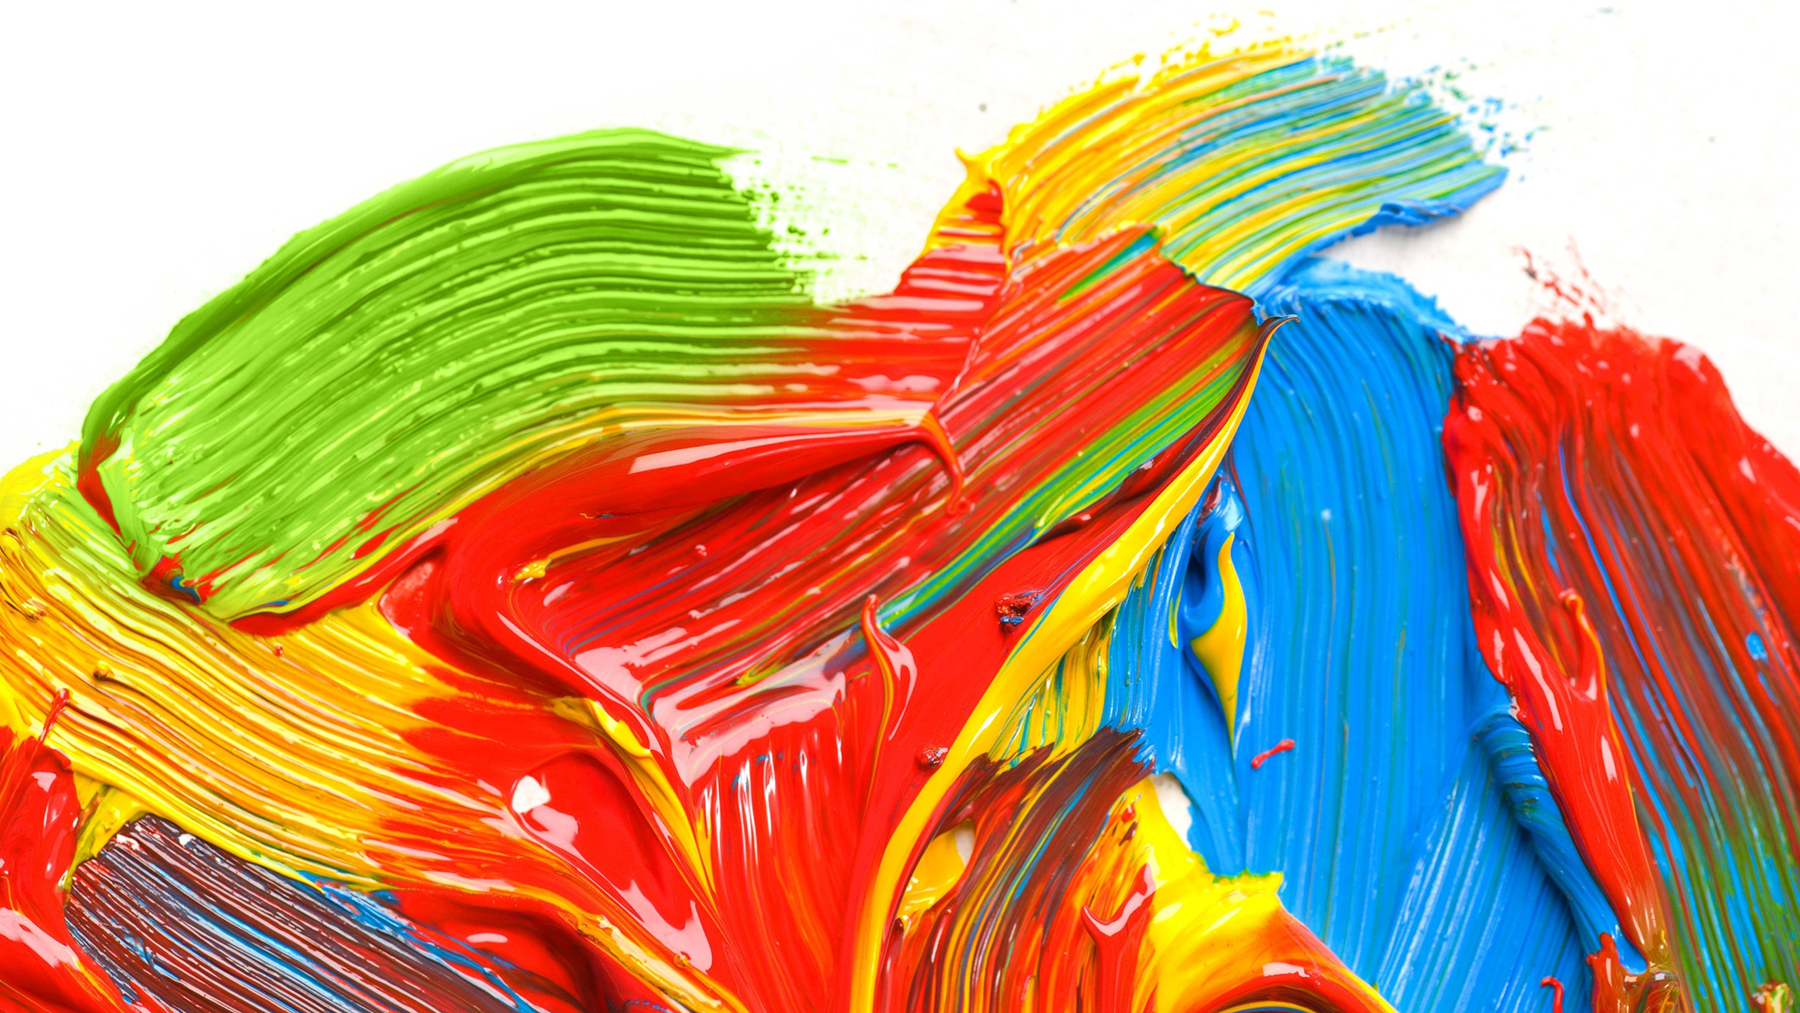
\includegraphics[width=1.1\paperwidth]{figs/paint-strokes_smaller.jpg}}
\begin{document}
% \maketitle

{\usebackgroundtemplate{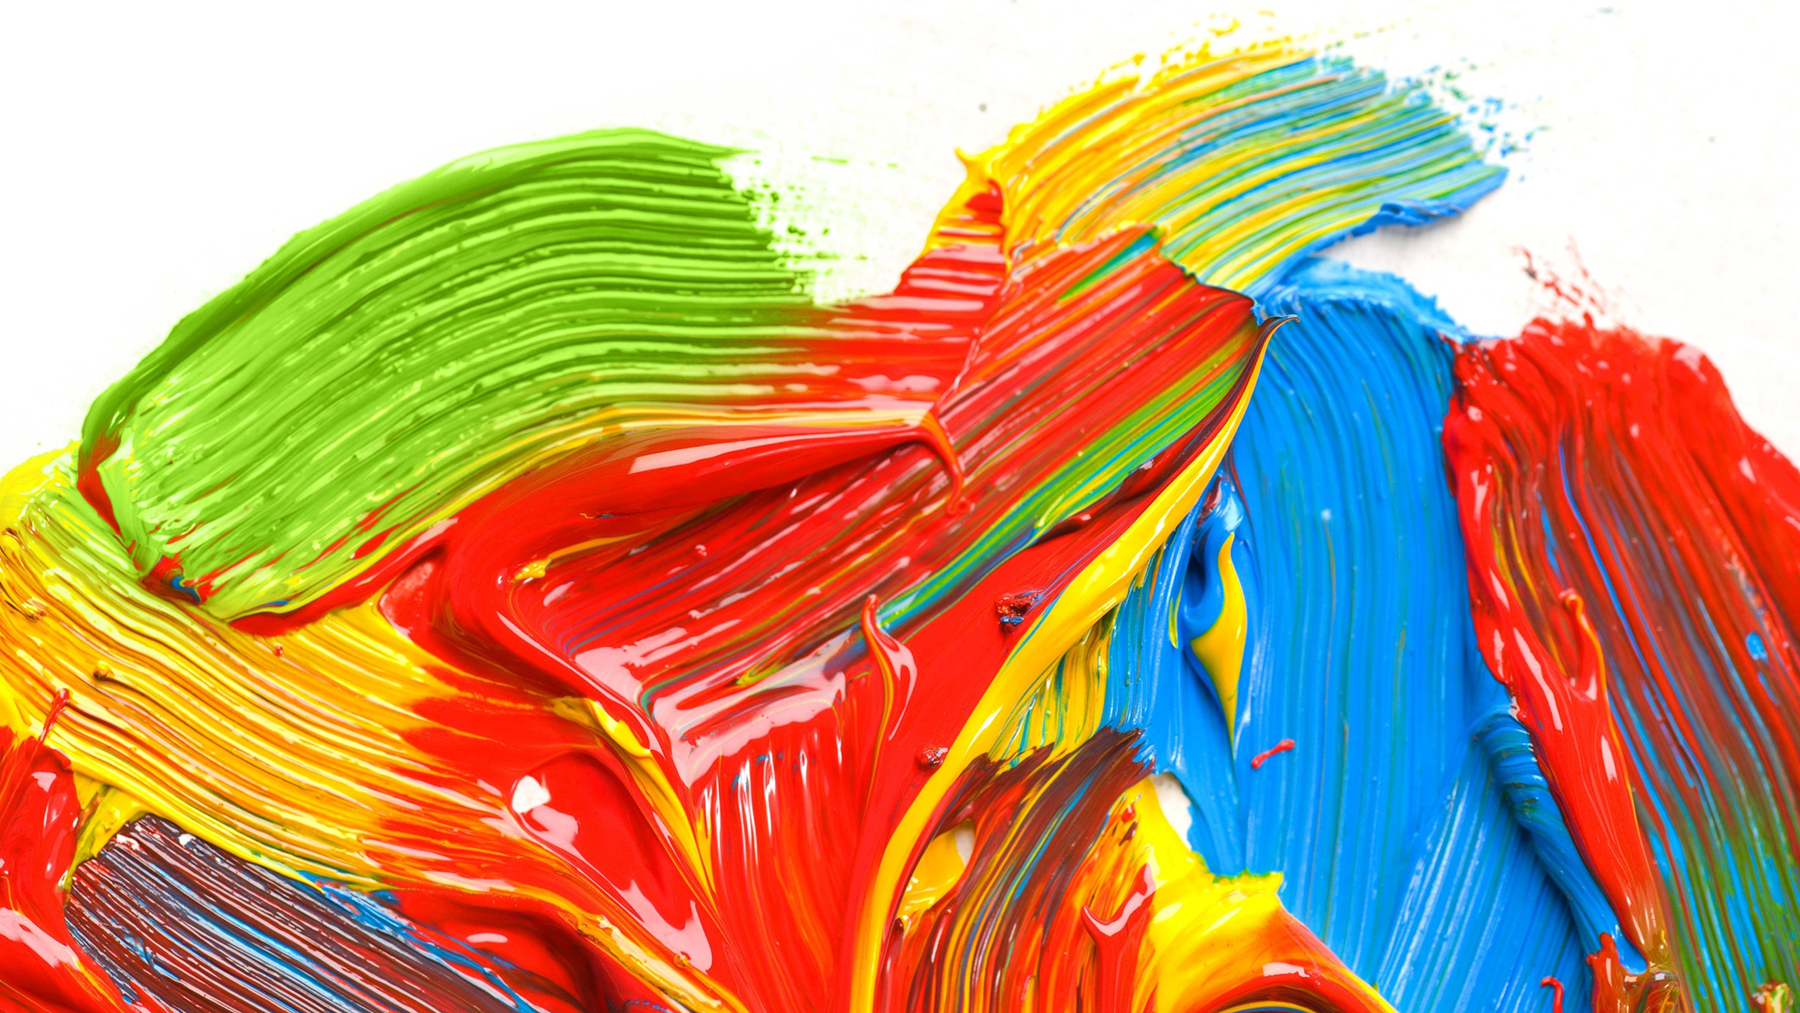
\includegraphics[width=\paperwidth]{figs/paint-strokes_smaller.jpg}}
\begin{frame}[plain]{}{}
    \titlepage
\end{frame}
}
% \section{Introduction}
    \begin{frame}[plain,noframenumbering]{}{}%{QCD world}
\centering
\vspace{5mm}\pause
Perspective of QCD -- large white space with little colorful objects\pause
\\\vspace{2cm}
% simple hadrons (baryons, mesons)\qquad
[zoom]\quad\quad\pause
\raisebox{-0.5\height}{\begin{overpic}[]{figs/atom2_ed.png}
    \put(0,-10) {atom}
    \put(10,110) {\centering$\xleftrightarrow[]{\qquad\,\,\sim 10\,\text{fm}\,\,\qquad}$}
\end{overpic}}\pause\qquad\qquad[zoom]\qquad\qquad\pause
\raisebox{-0.5\height}{\begin{overpic}[]{inline-figs/proton.pdf}
    \put(0,-12) {nucleon}
    \put(5,110) {\centering$\xleftrightarrow[]{\quad\,\,\sim 1\,\text{fm}\,\,\quad}$}
\end{overpic}}
% \raisebox{-0.5\height}{\begin{overpic}[]{inline-figs/neutron.pdf}
%     \put(0,-10) {neutron}
% \end{overpic}}
% \\\vspace{1cm}
% hadronic molecules (atoms)\qquad
% \raisebox{-0.5\height}{\begin{overpic}[]{inline-figs/deuteron.pdf}
%     \put(0,-5) {deuteron}
% \end{overpic}}\qquad{\Huge \dots\dots}
\end{frame}


\begin{frame}[plain]{}{}%{QCD world}
\centering
\vspace{5mm}%\pause
Perspective of QCD -- large white space with little colorful objects
\\\vspace{1cm}%\pause
simple hadrons (baryons, mesons)\qquad
\raisebox{-0.5\height}{\begin{overpic}[]{inline-figs/proton.pdf}
    \put(0,-10) {proton}
\end{overpic}} \qquad
\raisebox{-0.5\height}{\begin{overpic}[]{inline-figs/neutron.pdf}
    \put(0,-10) {neutron}
\end{overpic}} \qquad
\raisebox{-0.5\height}{\begin{overpic}[]{inline-figs/pion.pdf}
    \put(0,-10) {pion}
\end{overpic}}
\\\vspace{1cm}
hadronic molecules (atoms)\qquad
\raisebox{-0.5\height}{\begin{overpic}[]{inline-figs/deuteron.pdf}
    \put(0,-5) {deuteron}
\end{overpic}}\qquad{\Huge \dots\dots}
\end{frame}


\begin{frame}{If that's all, who are these?}{``Ok, google, show me known mesons'''...}
    \pause
    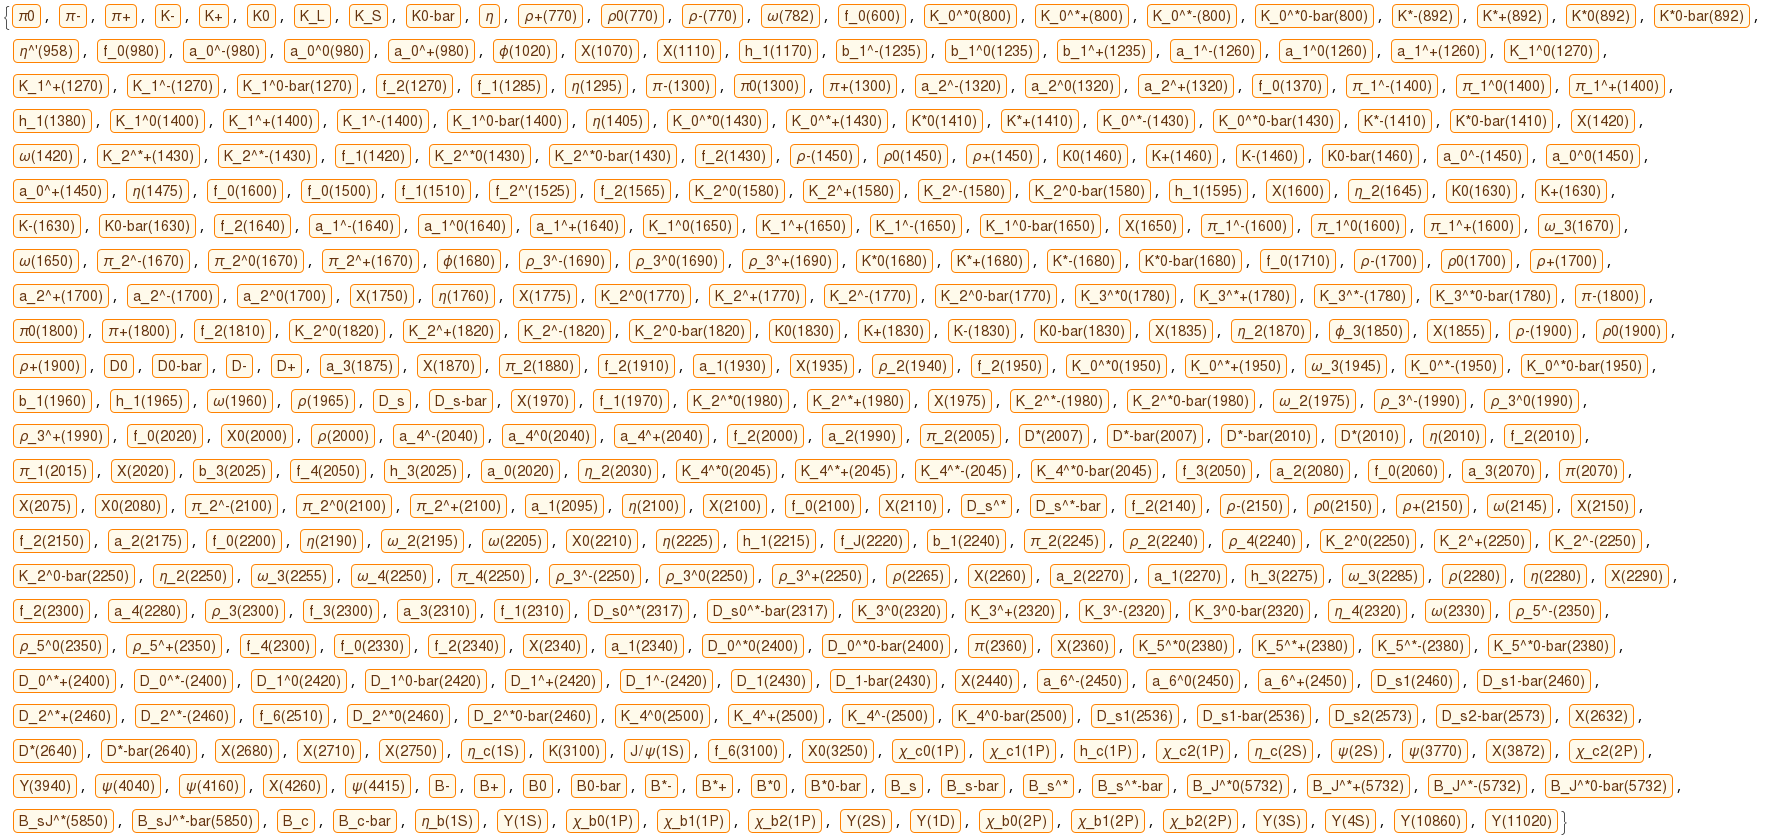
\includegraphics[width=0.95\textwidth]{figs/mesons-e.png}
\end{frame}

\definecolor{cola}{rgb}{0.9,0.62,0.0}
\newcommand{\baryon}[4]{
\begin{tikzpicture}[node distance=0.9cm and 1.3cm, baseline=-1cm]
  \node[coordinate] (a) at (-1,0) {};
  \filldraw[even odd rule,inner color=cola,outer color=white] (a) circle (1cm);
  \draw[black,thick] (a) circle (1cm);
  \draw[black] (a) ++(0.3,0.3) circle (3mm) node[] {#3};
  \draw[black] (a) ++(-0.4,0.1) circle (3mm) node[] {#2};
  \filldraw[even odd rule,inner color=quark,outer color=white] (a) ++(0,-0.5) circle (3mm);
  \draw[black, thick] (a) ++(0,-0.5) circle (3mm) node[] {#1};
  \draw[black] (a) ++(-1,-1) node[] {#4};
\end{tikzpicture}
}

\newcommand{\meson}[3]{
\begin{tikzpicture}[node distance=0.9cm and 1.3cm, baseline=-1cm]
  \node[coordinate] (a) at (-1,0) {};
  \filldraw[even odd rule,inner color=colb,outer color=white] (a) circle (1cm);
  \draw[black,thick] (a) circle (1cm);
  \draw[black] (a) ++(0.24,0.3) circle (3mm) node[] {#2};
  \filldraw[even odd rule,inner color=quark,outer color=white] (a) ++(-0.24,-0.4) circle (3mm);
  \draw[black, thick] (a) ++(-0.24,-0.4) circle (3mm) node[] {#1};
  \draw[black] (a) ++(-1,-1) node[] {#3};
\end{tikzpicture}
}

\newcommand{\quarkonia}[3]{
\begin{tikzpicture}[node distance=0.9cm and 1.3cm, baseline=-1cm]
  \node[coordinate] (a) at (-1,0) {};
  \filldraw[even odd rule,inner color=colb,outer color=white] (a) circle (1cm);
  \draw[black,thick] (a) circle (1cm);
  \filldraw[even odd rule,inner color=quark,outer color=white] (a) ++(0.24,0.3) circle (3mm);
  \draw[black, thick] (a) ++(0.24,0.3) circle (3mm) node[] {#2};
  \filldraw[even odd rule,inner color=quark,outer color=white] (a) ++(-0.24,-0.4) circle (3mm);
  \draw[black, thick] (a) ++(-0.24,-0.4) circle (3mm) node[] {#1};
  \draw[black] (a) ++(-1,-1) node[] {#3};
\end{tikzpicture}
}
% \begin{frame}{flavour modifications}
%     \begin{columns}
%         \begin{column}{0.5\textwidth}
%             \raisebox{-0.5\height}{
%             % \begin{overpic}[]{inline-figs/proton.pdf}
%                 % \put(0,-10) {$\Delta^{++}$}
%             % \end{overpic}}
%             \baryon}
%             \raisebox{-0.5\height}{
%             \begin{overpic}[]{inline-figs/proton.pdf}
%                 \put(0,-10) {$\Lambda$}
%             \end{overpic}}
%             \raisebox{-0.5\height}{
%             \begin{overpic}[]{inline-figs/proton.pdf}
%                 \put(0,-10) {$\Lambda_b$}
%             \end{overpic}}\\[8mm]
%             \raisebox{-0.5\height}{
%             \begin{overpic}[]{inline-figs/proton.pdf}
%                 \put(0,-10) {proton}
%             \end{overpic}}
%             \raisebox{-0.5\height}{
%             \begin{overpic}[]{inline-figs/proton.pdf}
%                 \put(0,-10) {$\Lambda$}
%             \end{overpic}}
%             \raisebox{-0.5\height}{
%             \begin{overpic}[]{inline-figs/proton.pdf}
%                 \put(0,-10) {$\Lambda_b$}
%             \end{overpic}}
%         \end{column}
%         \begin{column}{0.48\textwidth}
%             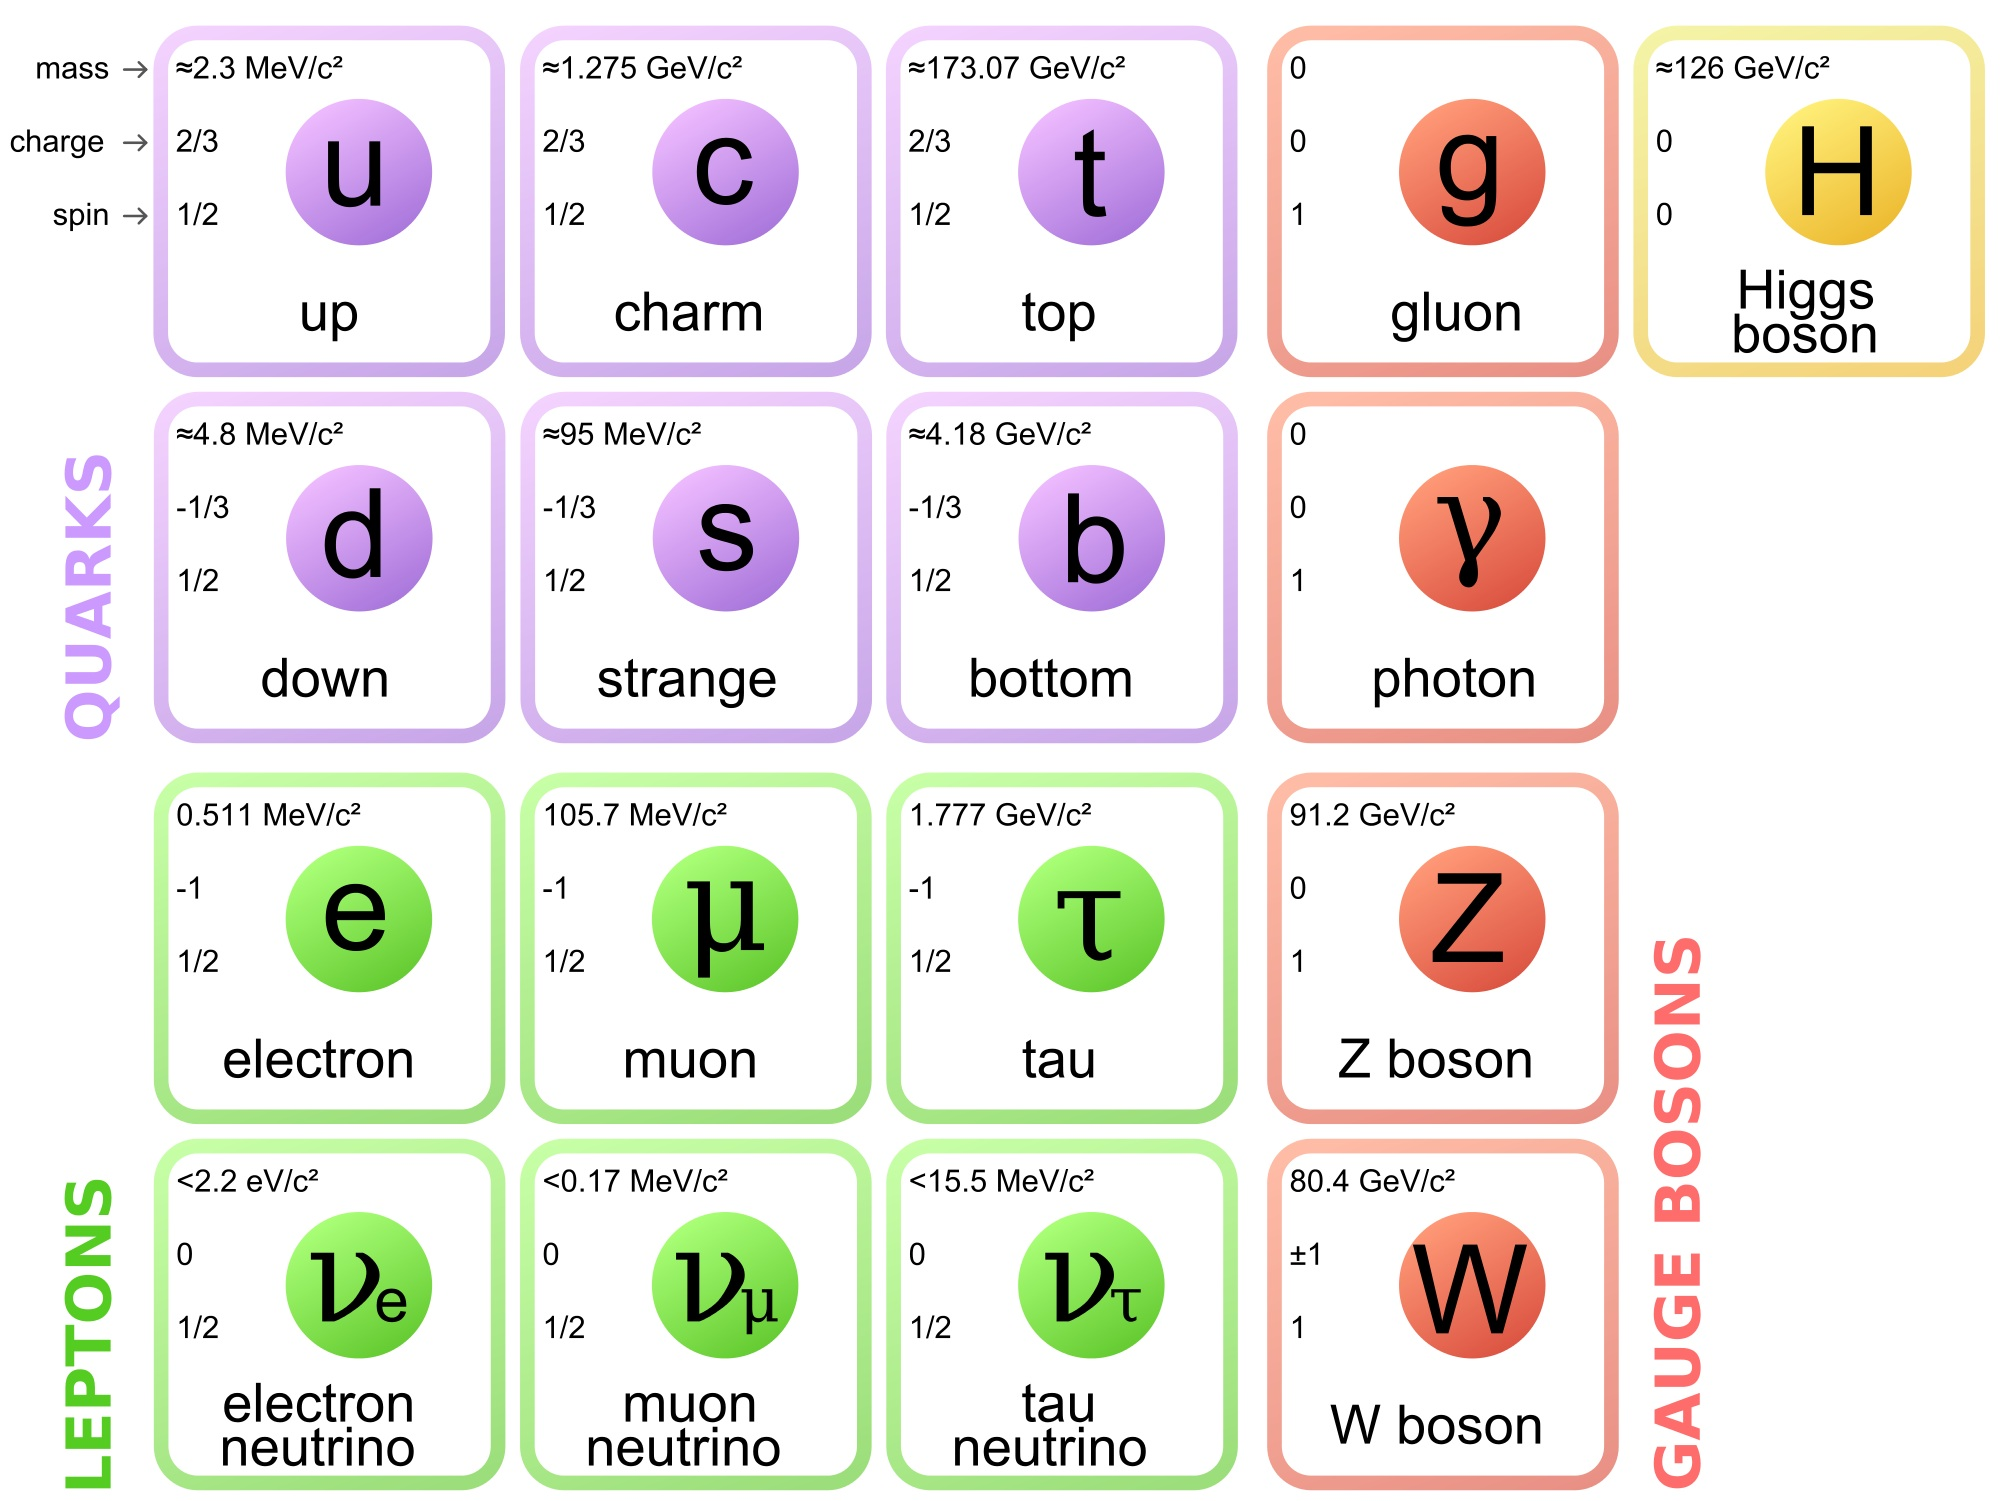
\includegraphics[width=\textwidth]{figs/SM_particles.jpg}
%         \end{column}
%     \end{columns}
% \end{frame}
\begin{frame}{Flavour modifications: Baryons}
    \begin{columns}
        \begin{column}{0.55\textwidth}
            \raisebox{-0.5\height}{\!\!\baryon{$u$}{$u$}{$d$}{$p$}}
            \raisebox{-0.5\height}{\!\!\baryon{$c$}{$u$}{$d$}{$\Lambda_c$}}\\
            % \raisebox{-0.5\height}{\!\!\baryon{$t$}{$u$}{$d$}{$\Lambda_t$}}\\
            \raisebox{-0.5\height}{\!\!\baryon{$d$}{$u$}{$d$}{$n$}}
            \raisebox{-0.5\height}{\!\!\baryon{$s$}{$u$}{$d$}{$\Lambda$}}
            \raisebox{-0.5\height}{\!\!\baryon{$b$}{$u$}{$d$}{$\Lambda_b$}}
        \end{column}
        \begin{column}{0.44\textwidth}
            \centering
            Standard Model particles\\[5mm]
            % \alt<2>{
            % \begin{overpic}[width=0.8\textwidth]{figs/flavour.png}
            %     \put(16,13) {\Huge $d$}
            %     \put(48,13) {\Huge $s$}
            %     \put(80,13) {\Huge $b$}
            %     \put(16,48) {\Huge $u$}
            %     \put(48,48) {\Huge $c$}
            %     \put(80,48) {\Huge $t$}
            % \end{overpic}
            \begin{overpic}[width=\textwidth]{figs/SM_particles_ed.jpg}
                \put(45,61) {\scalebox{4}{\color{red} $\times$}}
            \end{overpic}
        \end{column}
    \end{columns}
    \begin{exampleblock}{}
        All (ground) hadrons are stable without weak interaction
    \end{exampleblock}
\end{frame}

\begin{frame}[noframenumbering]{Flavour modifications: Mesons}
    \begin{columns}
        \begin{column}{0.55\textwidth}
            \raisebox{-0.5\height}{\!\!\meson{$u$}{$\bar{u}$}{$\pi$}}
            \raisebox{-0.5\height}{\!\!\meson{$c$}{$\bar{u}$}{$D$}}\\
            % \raisebox{-0.5\height}{\!\!\meson{$t$}{$\bar{u}$}{$\Lambda_t$}}\\
            \raisebox{-0.5\height}{\!\!\meson{$d$}{$\bar{u}$}{$\pi$}}
            \raisebox{-0.5\height}{\!\!\meson{$s$}{$\bar{u}$}{$K$}}
            \raisebox{-0.5\height}{\!\!\meson{$b$}{$\bar{u}$}{$B$}}
        \end{column}
        \begin{column}{0.44\textwidth}
            \centering
            Standard Model particles\\[5mm]
            \begin{overpic}[width=\textwidth]{figs/SM_particles_ed.jpg}
                \put(45,61) {\scalebox{4}{\color{red} $\times$}}
            \end{overpic}
        \end{column}
    \end{columns}
    \begin{exampleblock}{}
        All (ground) hadrons are stable without weak interaction
    \end{exampleblock}
\end{frame}

\begin{frame}[noframenumbering]{Flavour modifications: Flavour-neutral Mesons}
    \begin{columns}
        \begin{column}{0.55\textwidth}
            \raisebox{-0.5\height}{\!\!\quarkonia{$u$}{$\bar{u}$}{$\pi$}}
            \raisebox{-0.5\height}{\!\!\quarkonia{$c$}{$\bar{c}$}{$J/\psi$}}\\
            % \raisebox{-0.5\height}{\!\!\quarkonia{$t$}{$\bar{u}$}{$\Lambda_t$}}\\
            \raisebox{-0.5\height}{\!\!\quarkonia{$d$}{$\bar{d}$}{$\pi$}}
            \raisebox{-0.5\height}{\!\!\quarkonia{$s$}{$\bar{s}$}{$\phi$}}
            \raisebox{-0.5\height}{\!\!\quarkonia{$b$}{$\bar{b}$}{$\Upsilon$}}
        \end{column}
        \begin{column}{0.44\textwidth}
            \centering
            Standard Model particles\\[5mm]
            \begin{overpic}[width=\textwidth]{figs/SM_particles_ed.jpg}
                \put(45,61) {\scalebox{4}{\color{red} $\times$}}
            \end{overpic}
        \end{column}
    \end{columns}
    \begin{exampleblock}{}
        All (ground-state) hadrons are stable without the weak interaction
    \end{exampleblock}
\end{frame}

\begin{frame}{Conventional states: why so many hadrons}{}
    % \vspace{-5mm}
    \begin{overpic}[width=0.7\textwidth]{figs/quark_model_charmonium_ed.png}
        \put(72,0) {\parbox{\textwidth}{
            Isovector meson spectrum with $m_\pi\sim 800\,\text{MeV}$\\
            \paper{J.~Dudek et al., PRD82 034508 (2010)}}}
        \put(110,40) {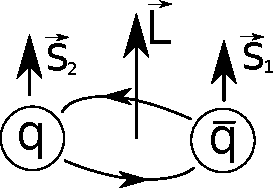
\includegraphics[width=0.2\textwidth]{figs/LS_qqbar.pdf}}
        \put(72,35) {
        \begin{minipage}[t]{0.48\textwidth}
            \begin{exampleblock}{Hadronic states - energy levels}
                \begin{itemize}
                    \item Orbital excitation, $\vec L$
                    \item Radial excitation, $n$
                    \item Spin-orbit interaction, $\vec J = \vec L \oplus \vec S$
                \end{itemize}
            \end{exampleblock}
            \end{minipage}
        }
        \only<2>{
        \put(48,08) {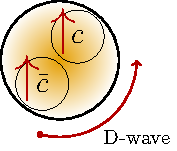
\includegraphics[width=0.1\textwidth]{inline-figs/MesonCC.pdf}}
        \put(28,02) {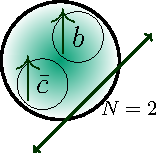
\includegraphics[width=0.095\textwidth]{inline-figs/MesonBC.pdf}}
        \put(50,18) {\color{red} \vector(-0.5,1){9}}
        \put(30,12) {\color{red} \vector(-0.6,1){12}}
        \put(50,24) {\paper{LHCb (2019)}}
        \put(30,18) {\paper{LHCb (2019)}}
        }
        % \put(30,20) {\color{red} \circle{5}}
        % \put(10,20) {\color{red} \vector(0,1){5}}
    \end{overpic}
\end{frame}

\begin{frame}{Hadrons: every flavour gets its energy range\hfill\paper{PDG2019}}
    \vspace{3mm}
    \begin{columns}
        \begin{column}{0.7\textwidth}
            \alt<2>{
            \begin{overpic}[width=\textwidth]{figs/rpp2018-sigma_R_ee_ed.pdf}
                    \put( 67,10)  {SM Sector ($Z$, $W$, $H$)}
                    % \put( 65,13)  {\color{red}\vector(1,0){40}}
            \end{overpic}
            }{
            \begin{overpic}[width=\textwidth]{figs/rpp2018-sigma_R_ee.pdf}
                    % \put( 67,10)  {SM Sector ($Z$, $W$, $H$)}
                    % \put( 65,13)  {\color{red}\vector(1,0){40}}
                \end{overpic}
            }
        \end{column}
        \begin{column}{0.29\textwidth}
            \vspace{-3mm}
            \begin{block}{$R$-ratio}
                \!\!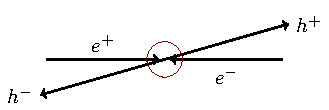
\includegraphics[width=\textwidth]{inline-figs/collision_ee.pdf}
                $$R = \frac{e^+e^-\to\textrm{hadrons}}{e^+e^-\to\mu^+\mu^-}$$
                $\textrm{hadrons}:\,h^+h^-,\dots$
            \end{block}
        \end{column}
    \end{columns}\pause
    \vspace{-2mm}
    \begin{itemize}
        \item {\color{cola} Light (contain $u$,$d$,$s$)}\quad
        {\color{colb} Hidden charmed ($c\bar{c}$)}\quad
        {\color{colc} Hidden beauty ($b\bar{b}$)}\pause
        \item Energy ranges do not overlap
    \end{itemize}
    \vspace{-2mm}
    \begin{exampleblock}{}
        $\Rightarrow$ Energy range tells the flavour
    \end{exampleblock}
\end{frame}

\section{LHCb experiment}

\begin{frame}[plain]{\color{black} Search for the new type of matter\small\hfill\href{http://clangenb.web.cern.ch/clangenb/}{\color{orange}[link]}}
    {\color{black}How to search for color physics with colorless environment?}
\centering
\begin{overpic}[width=0.75\textwidth]{figs/lhcb_detector_bw.png}
    % \put(40,55) {}
    \put(-10,50) {\Huge \textbf{LHCb}}
    \put(60,-3) {\tiny modification of a plot from {\tiny [INT. J. MOD. PHYS. A 30, 1530022]}}
    \put(-5,28) {\large $7\,$TeV}
    \put(100,28) {\large $7\,$TeV}
    \put(15,27.5) {\thicklines \color{red}\circle{5}}
    \put(78,55) {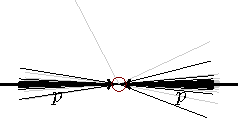
\includegraphics[width=0.3\textwidth]{inline-figs/collision_pp.pdf}}
\end{overpic}
\end{frame}

\section{Pentaquarks}

% \begin{frame}[plain,noframenumbering]{}
% \begin{center}
%     \Huge Pentaquark states $P_c$
%     \\[2cm]
%     \Large Hadronic molecules\qquad$\xLeftrightarrow[]{\quad???\quad}$\qquad
%     \raisebox{-0.5\height}{
%     \begin{overpic}[scale=1.5]{inline-figs/pentaquarks.pdf}
%         \put( -5,0) {\LARGE $\bar{D}^0$}
%         \put(95,0) {\LARGE $\Sigma_c^+$}
%     \end{overpic}}
% \end{center}
% % Perhaps, like $J/\psi$ but excited.
% \end{frame}

{\usebackgroundtemplate{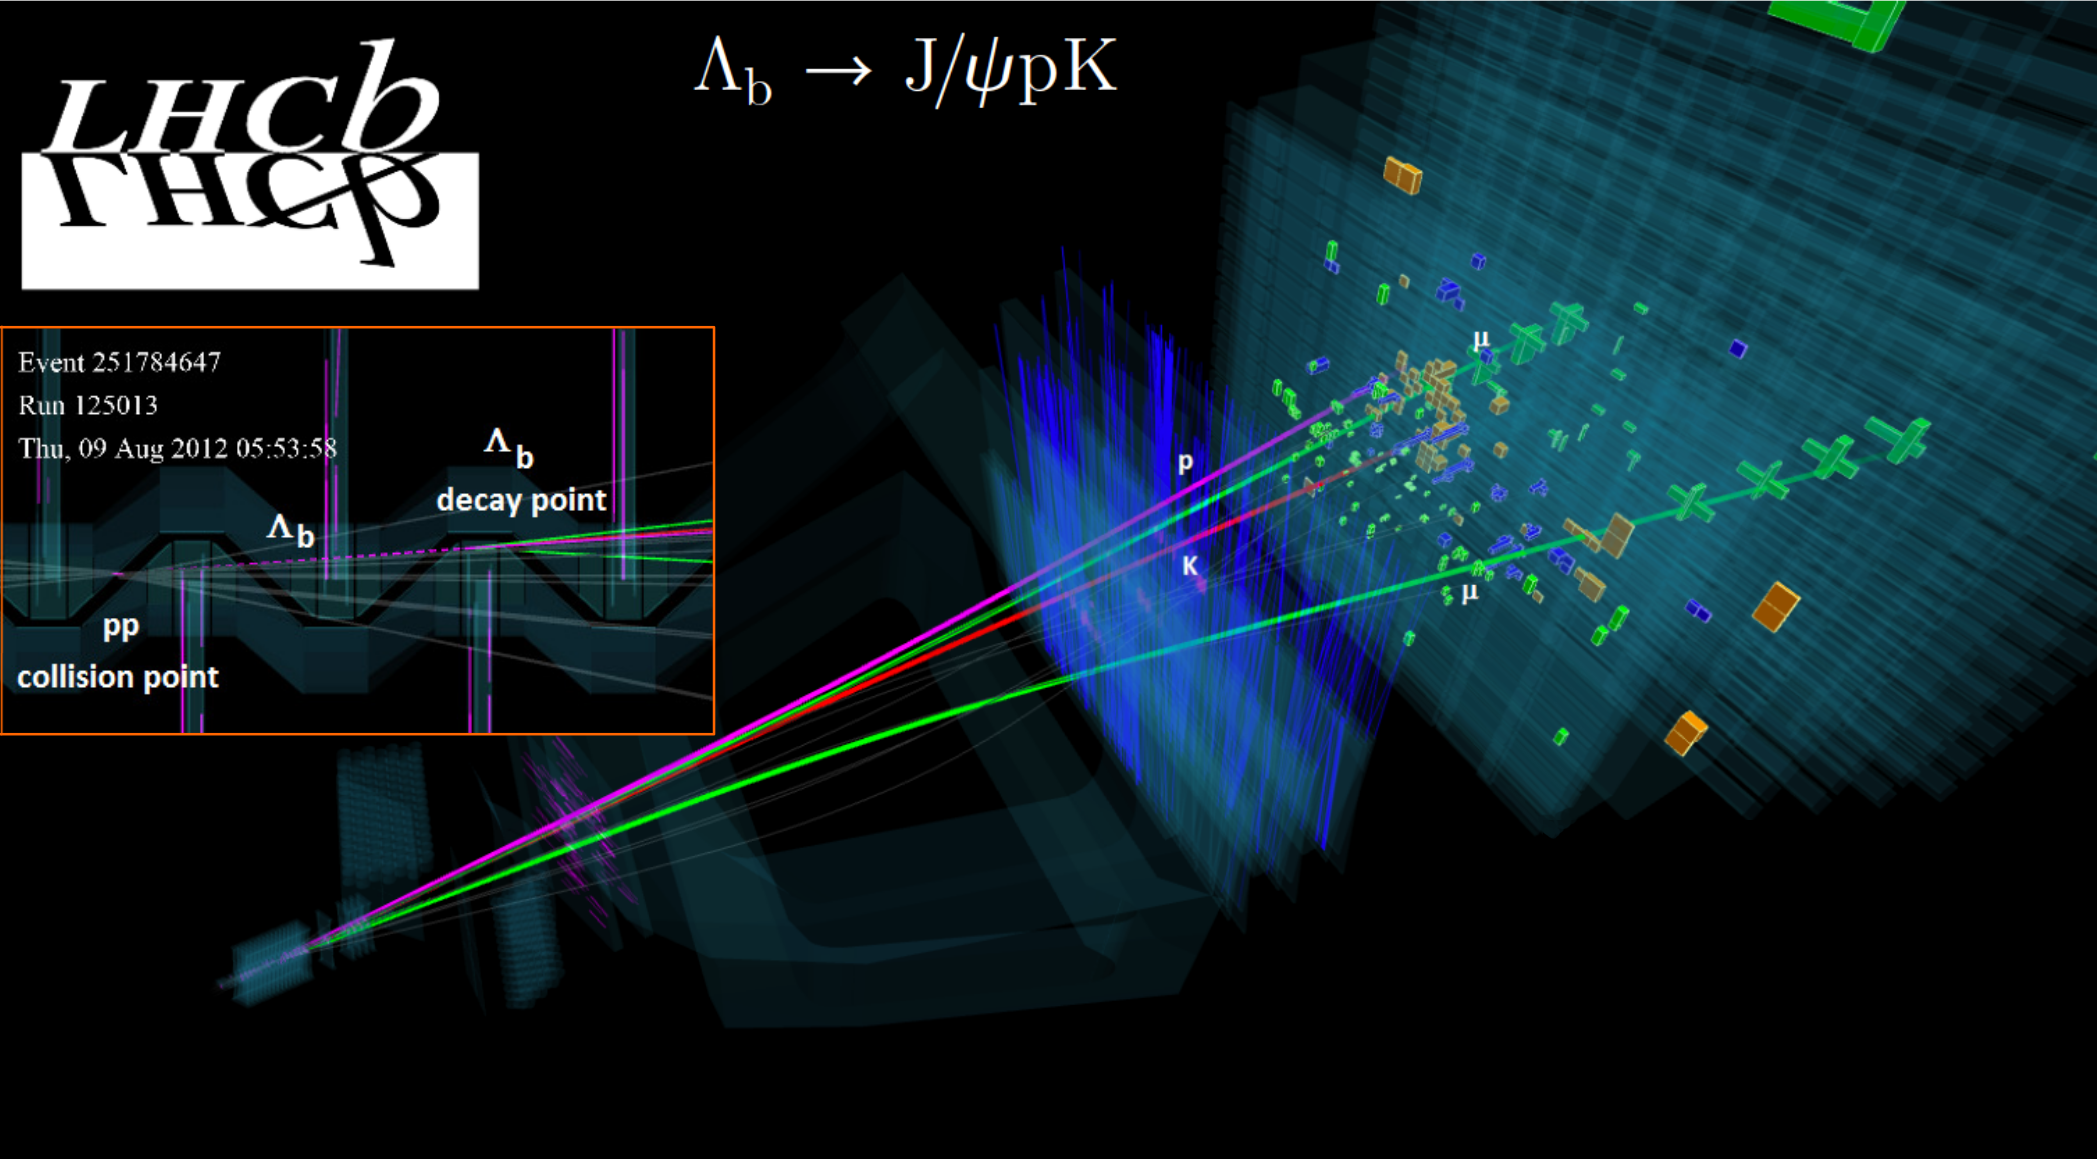
\includegraphics[width=\paperwidth]{figs/event_display_ed1.png}}
\begin{frame}[plain]{}{}
    % \titlepage
\end{frame}
}

\begin{frame}{Almost-stable hadrons}{Lifetime measurements of $\Lambda_b^0$ and $B^0$}
\begin{columns}
    \begin{column}{0.45\textwidth}
        \begin{itemize}
            \item identification of displaced vertex\\
            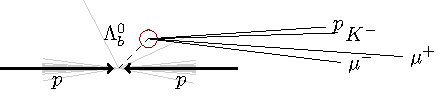
\includegraphics[scale=0.85]{inline-figs/collision.pdf}\\
            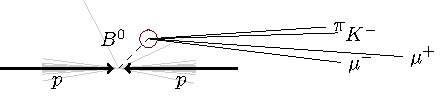
\includegraphics[scale=0.85]{inline-figs/collision_to_B0.pdf}
            \item similar decay chains
        \end{itemize}
        \centering
        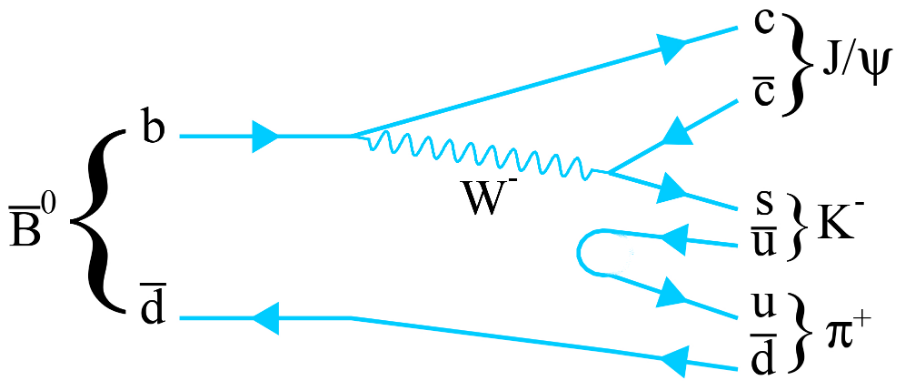
\includegraphics[width=0.49\textwidth]{figs/Lifetime/diagram_B.png}
        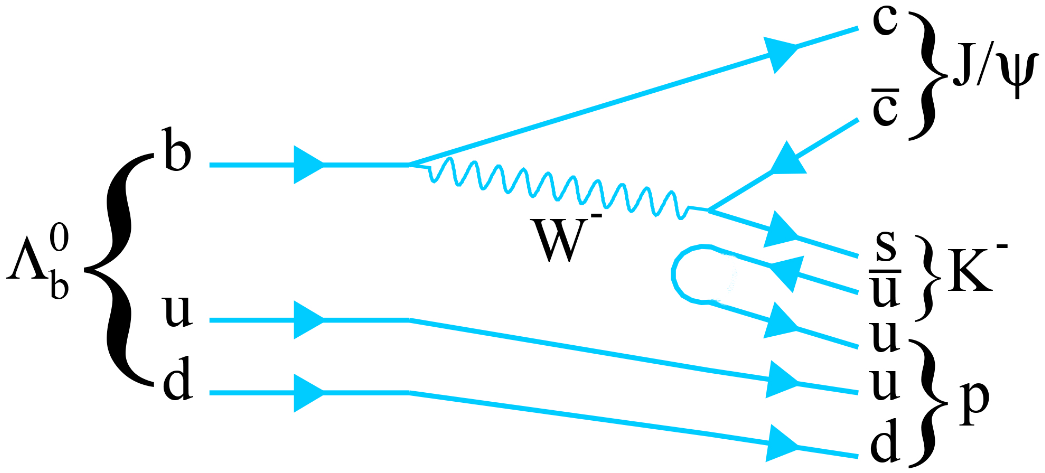
\includegraphics[width=0.49\textwidth]{figs/Lifetime/diagram_Lb.png}
        % \begin{exampleblock}{Measurements of proper time}
        %     \begin{itemize}
        %         \item secondary displaced vertex
        %         \item
        %     \end{itemize}
        %     % 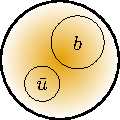
\includegraphics[width=0.3\textwidth]{inline-figs/Meson.pdf}
        %     % 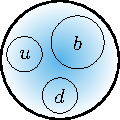
\includegraphics[width=0.3\textwidth]{inline-figs/Baryon.pdf}
        % \end{exampleblock}
    \end{column}\pause
    \begin{column}{0.5\textwidth}
        \begin{overpic}[width=\textwidth]{figs/Lifetime/Yield.pdf}
            \put(20,16) {\color{red}$Y(t)\sim e^{-t/\tau}$}
            \put(60,46) {\color{green!50!black}$B^0$\quad\raisebox{-0.5\height}{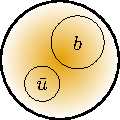
\includegraphics[width=8mm]{inline-figs/Meson.pdf}}}
            \put(30,30) {\raisebox{-0.5\height}{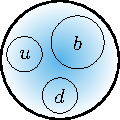
\includegraphics[width=8mm]{inline-figs/Baryon.pdf}}\,\,
                        \color{blue}$\Lambda_b^0$}
            \put(78,56) {\color{blue} @$3\,$fb$^{-1}$}
            \put(60,66) {\scriptsize [PLB734 (2014) 122]}
        \end{overpic}
        \centering
        $\tau_{\Lambda_b^0}/\tau_{B^0} = 0.974\pm 0.006\pm 0.004,$\\[2mm]
        \framebox{
        $\tau_{\Lambda_b^0} = 1.479\pm 0.009\pm 0.010\,$ps,}\\
        % still the smallest statistical error!
    \end{column}
\end{columns}
\end{frame}
%
% \begin{frame}{$P_c(4450)$ in the decay $\Lambda_b^0\to J/\psi\,p\,K$ \hfill \paper{Phys.Rev.Lett. 115}}
%   \vspace{2mm}
%   \begin{columns}
%     \begin{column}{0.6\textwidth}
%       \begin{overpic}[width=0.7\textwidth]{figs/PcOld/dlz.pdf}
%         \put (98,67) {\rotatebox{-90}{\scalebox{-1}[1]{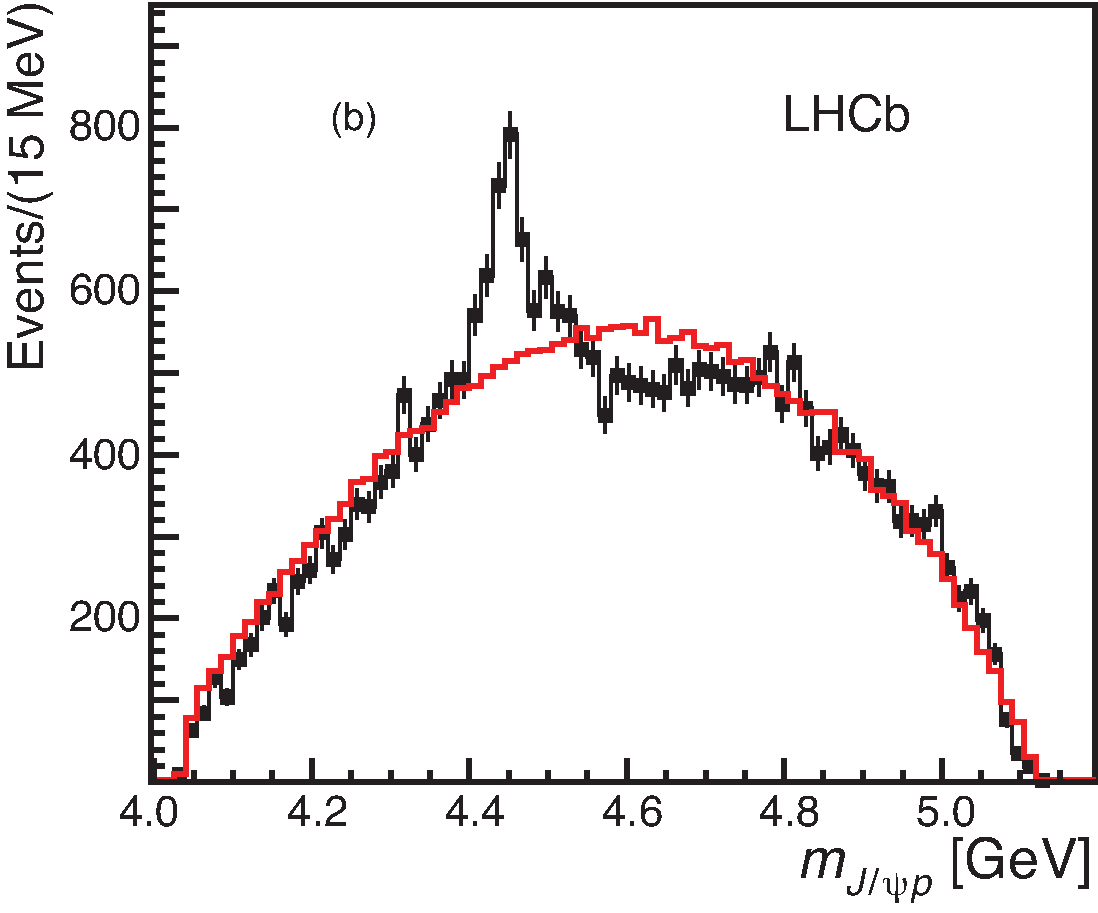
\includegraphics[width=0.46\textwidth]{figs/PcOld/mjpsip-phsp.pdf}}}}
%         \put (155,70) {\rotatebox{-90}{\scalebox{-1}[1]{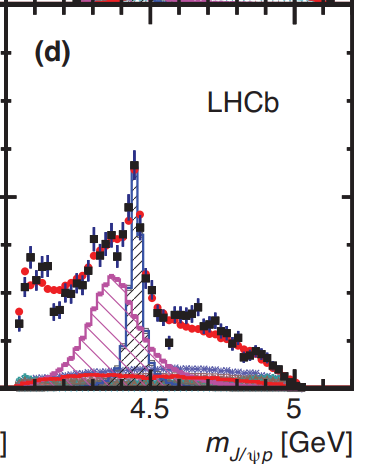
\includegraphics[width=0.38\textwidth]{figs/PcOld/Pc_proj.png}}}}
%         \put (0,-60) { 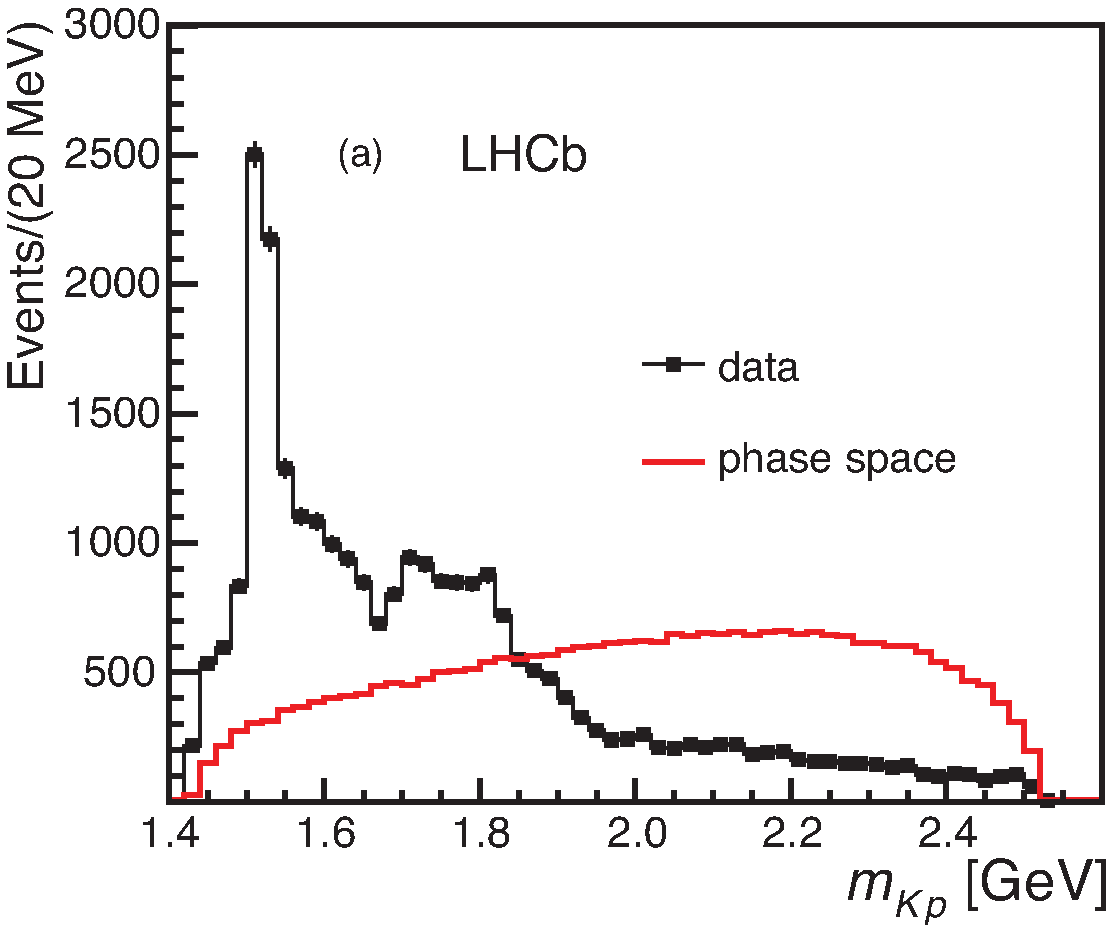
\includegraphics[width=0.6\textwidth]{figs/PcOld/mkp-phsp.pdf}}
%       \end{overpic}
%     \end{column}
%     \begin{column}{0.32\textwidth}
%     \end{column}
%   \end{columns}
%   \vspace{-1.5mm}
% \begin{columns}
%   \begin{column}{0.43\textwidth}
%   \end{column}
%   \begin{column}{0.55\textwidth}
%     \begin{exampleblock}{}
%       \begin{itemize}
%         \item High significance of pentaquark signals
%         \item The extracted quantum number $(3/2^-,5/2^+)$ are ambiguous.
%         \item The parameters rely on description of the $pK$ channel.
%       \end{itemize}
%     \end{exampleblock}
%   \end{column}
% \end{columns}
% \end{frame}
%
% % \begin{frame}[plain,noframenumbering]{}{}
% % \centering
% % \includegraphics[width=\textwidth]{}
% % \end{frame}
%

\begin{frame}{Dynamics of the decay $\Lambda_b^0\to J/\psi\,p\,K$,\hfill \scriptsize[PRL 115, 072001 (2015)]}{}%{ }
\begin{columns}
    \begin{column}{0.6\textwidth}
        \begin{exampleblock}{}
            Highly non-trivial transition amplitude
            \begin{itemize}
                \item interaction in $pK$ subsystem
                \item something in $J/\psi p$ subsystem (!?)
            \end{itemize}
        \end{exampleblock}
    \end{column}
    \begin{column}{0.38\textwidth}
        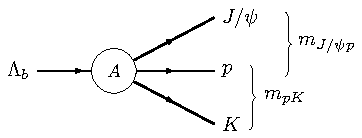
\includegraphics[width=0.9\textwidth]{inline-figs/Penta_decay_indication.pdf}
    \end{column}
\end{columns}
\centering
\alt<2>{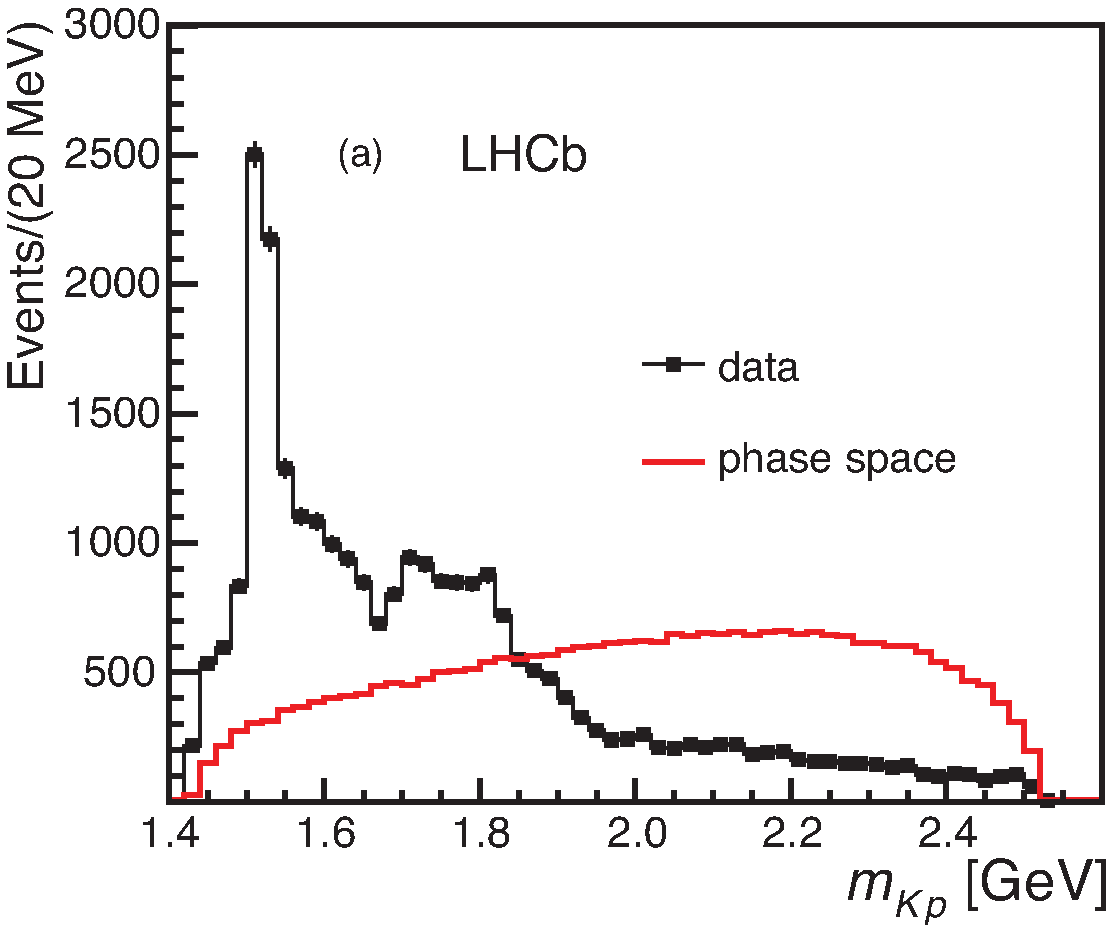
\includegraphics[width=0.43\textwidth]{figs/PcOld/mkp-phsp.pdf}}
{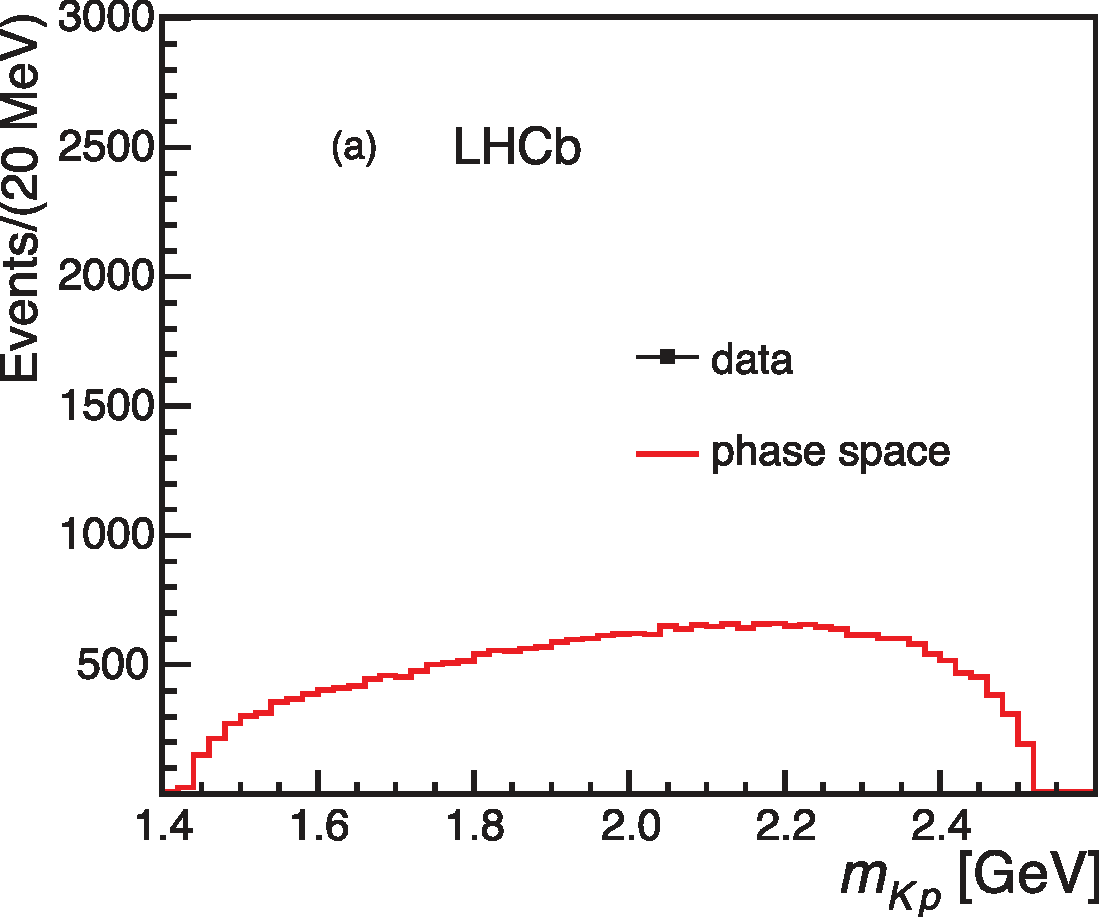
\includegraphics[width=0.43\textwidth]{figs/PcOld/mkp-phsp_phase_space.pdf}}
\alt<2>{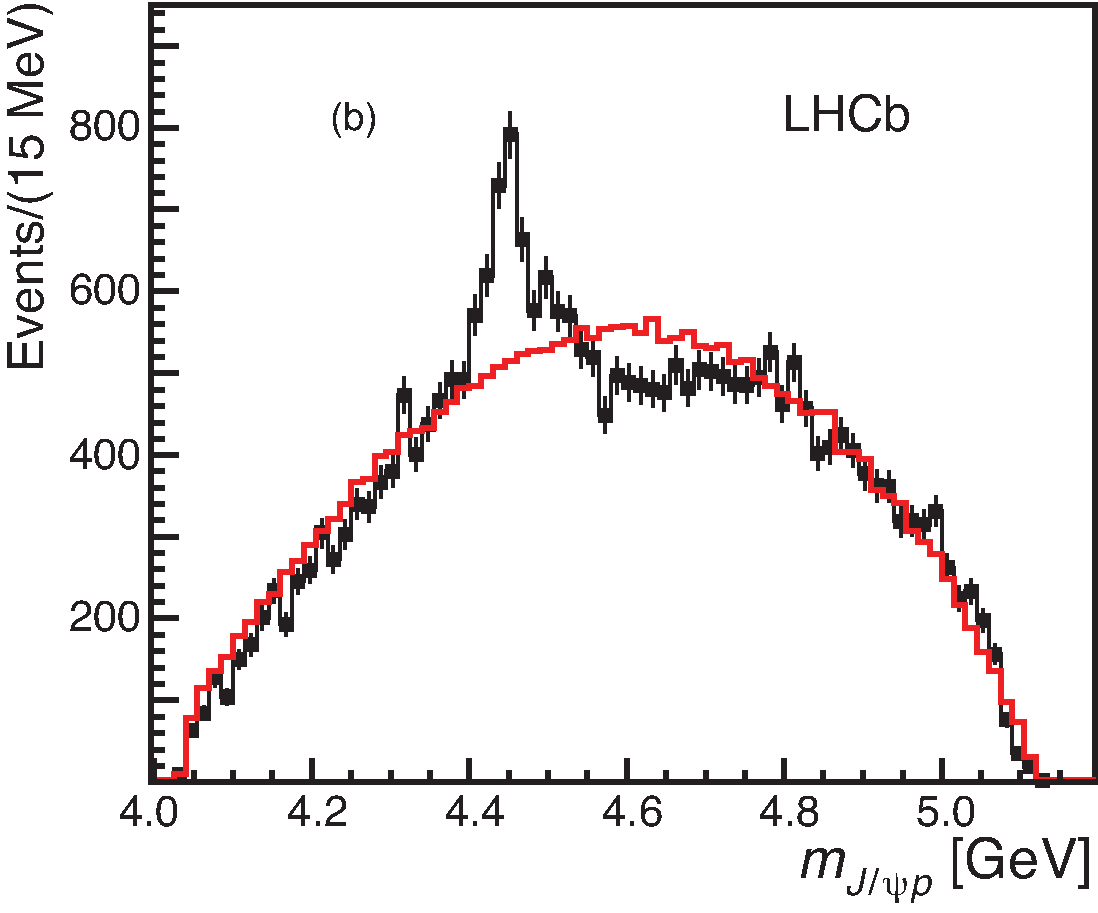
\includegraphics[width=0.43\textwidth]{figs/PcOld/mjpsip-phsp.pdf}}
{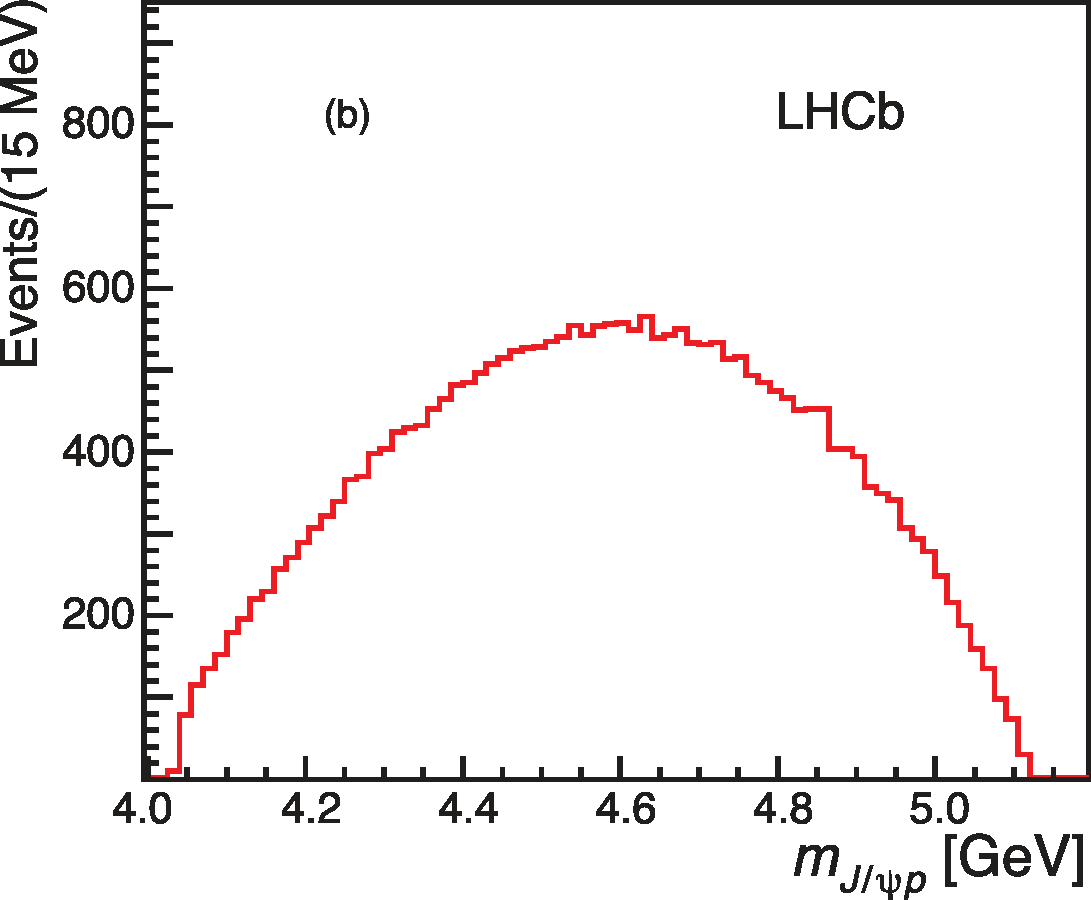
\includegraphics[width=0.43\textwidth]{figs/PcOld/mjpsip-phsp_phase_space.pdf}}
\end{frame}

\begin{frame}{What could we expect}
    \begin{center}
        \Huge Example demo\\[1cm]
        \raisebox{-0.5\height}{
\includegraphics[width=0.3\textwidth]{figs/julia-logo-300.png}}\qquad
        \raisebox{-0.5\height}{
\includegraphics[width=0.25\textwidth]{figs/atom_ed.png}}
    \end{center}
\end{frame}

\begin{frame}{Observation of $P_c(4450)$ and $P_c(4380)$,\hfill \scriptsize[PRL 115, 072001 (2015)]}{}%{ }
\begin{columns}
    \begin{column}{0.58\textwidth}
    \vspace{-2mm}
    \begin{center}
        \begin{overpic}[width=0.7\textwidth]{figs/PcOld/dlz.pdf}
            \put (105,32) {\color{red}\thicklines\vector(-1,0){10}\,\scriptsize $P_c(4450)$}
            \put (100,25) {\color{red}$\sim$\,\scriptsize $P_c(4380)$}
            \put(70,50) {\color{blue} @$3\,$fb$^{-1}$}
        \end{overpic}
    \end{center}
    \vspace{-5mm}
    \begin{block}{Amplitude analysis of 2015}
        % Isobar model:
        Helicity formalism, isobar model, $6$-dim. analysis.\\
        \vspace{-7mm}
        $$
        \raisebox{-0.5\height}{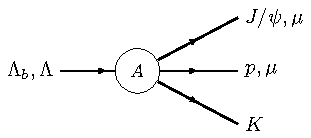
\includegraphics[scale=0.5]{inline-figs/Penta_decay.pdf}} =
        % \underbrace{
        \raisebox{-0.5\height}{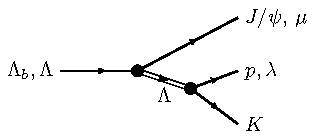
\includegraphics[scale=0.5]{inline-figs/Penta_isobar_23.pdf}}
        % }_{14\,\Lambda\,\text{states}} +
        % \underbrace{
        \raisebox{-0.5\height}{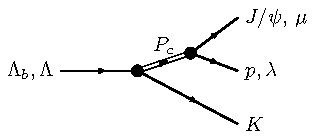
\includegraphics[scale=0.5]{inline-figs/Penta_isobar_12.pdf}}
        % }_{2\,\text{pentaquark states}}
        $$
        \vspace{-2mm}\\
        $\Rightarrow$ first ever observation of 5-quark states $[uudc\bar{c}]$.
    \end{block}
    % \begin{center}
    %     \begin{overpic}[height=0.27\textheight]{figs/Pc_molecule.png}
    %     \end{overpic}
    %     \begin{overpic}[height=0.27\textheight]{figs/Pc_tigthly-bound.png}
    %     \end{overpic}
    % \end{center}
    \end{column}
    \begin{column}{0.4\textwidth}
        \begin{overpic}[width=0.47\textwidth]{figs/PcOld/mjpsip-extendedNoPc.pdf}
            \put(20,77) {\tiny No pentaquarks}
        \end{overpic}
        \begin{overpic}[width=0.47\textwidth]{figs/PcOld/mjpsip-extended1Pc.pdf}
            \put(20,77) {\tiny One pentaquarks}
        \end{overpic}\\
        \begin{overpic}[width=\textwidth]{figs/PcNew/FigCDS2a.pdf}
            \put(50,75) {\scriptsize Two pentaquarks}
        \end{overpic}
    \end{column}
\end{columns}
\end{frame}

\begin{frame}{Adding more data with Run-II (2017,2018)\hfill\scriptsize[arXiv:1904.03947]}
\begin{columns}
\begin{column}{0.33\textwidth}
    \alt<1>{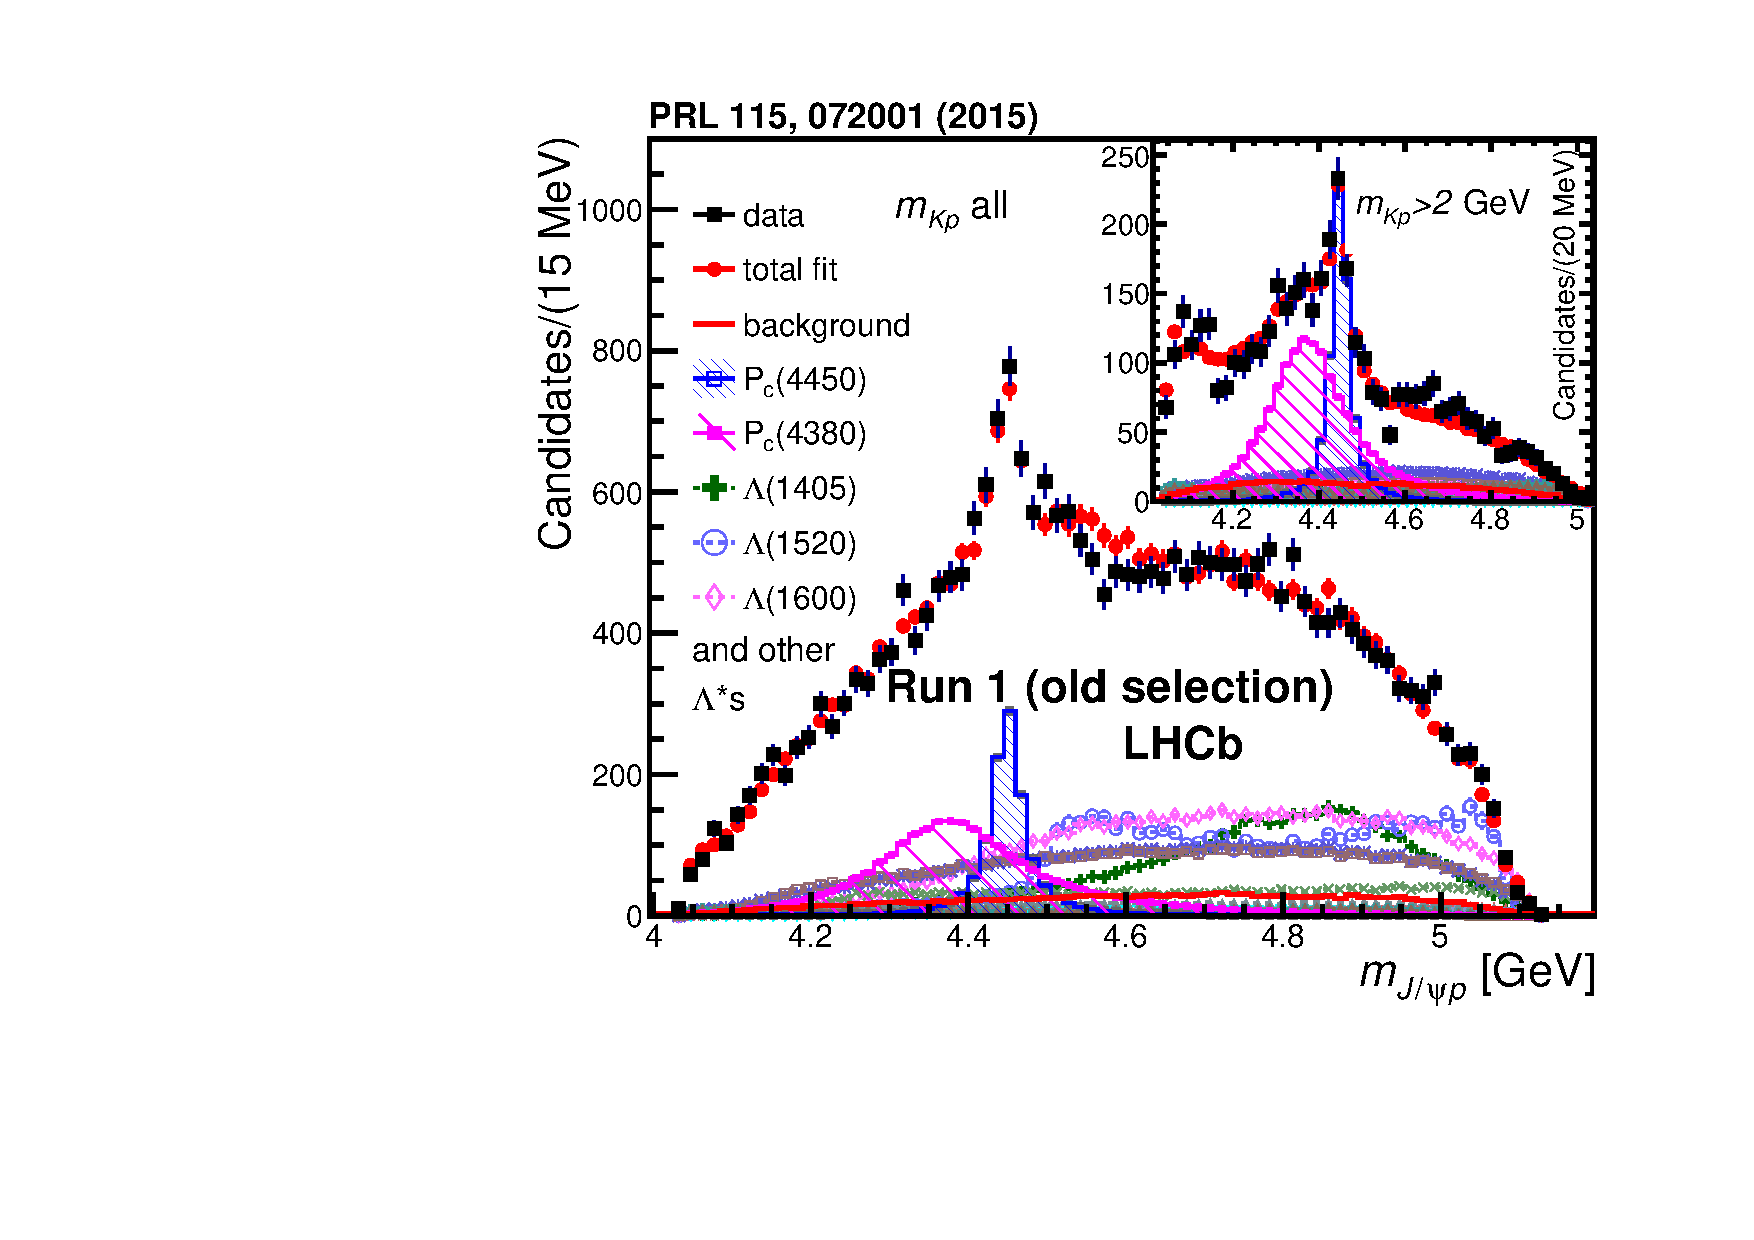
\includegraphics[width=\textwidth]{figs/PcNew/FigCDS2a.pdf}}
    {\begin{overpic}[width=\textwidth]{figs/PcNew/FigCDS2b.pdf}
            % \put(10,100) {\prt}
    \end{overpic}}
    \alt<1>{
    \begin{overpic}[width=\textwidth]{figs/PcOld/dlz.pdf}
        \put (75,32) {\color{red}\thicklines\vector(-1,0){10}\,\tiny $P_c(4450)$}
        \put (75,25) {\color{red}$\sim$\tiny $P_c(4380)$}
        \put(70,50) {\color{blue} \scriptsize @$3\,$fb$^{-1}$}
    \end{overpic}
    }{
    \begin{overpic}[width=\textwidth]{figs/PcNew/Dalitz_plot_pc.pdf}
        \put (75,36) {\color{blue!70!black}\thicklines\vector(-1,0){10}\,\tiny $P_c(445?)$}
        \put (75,29) {\color{green!70!black}\thicklines\vector(-1,0){10}\,\tiny $P_c(4312)$}
        \put(60,70) {\color{blue} \scriptsize @$9\,$fb$^{-1}$}
    \end{overpic}
    }
\end{column}\pause
\begin{column}{0.33\textwidth}
\begin{block}{Gain in statistics $\times 9$}
    \scriptsize
    $26k\text{ events}\Rightarrow\,246k\text{ events}$
    \begin{itemize}
        \item Luminosity: $3\,$fb$^{-1}\oplus 6\,$fb$^{-1}$,
        \item Cross section $\times 2$: $7\,$TeV$\to 13\,$TeV,
        \item Selection efficiency $\times 2$.
    \end{itemize}
\end{block}
\begin{exampleblock}{Amplitude Analysis}
    % \scriptsize
    \begin{itemize}
        \item same AA gives consistent results,
        \item but unacceptable quality.
        \begin{itemize}
            \item Narrow peaks in $J/\psi p$
            \item Lineshape of $\Lambda$.
        \end{itemize}
    \end{itemize}
\end{exampleblock}
\end{column}
\begin{column}{0.25\textwidth}
    \pause
    \begin{overpic}[width=1.1\textwidth]{figs/PcNew/mjpsip-spectrum-all-ed.pdf}
        \put (34,48) {\color{green!70!black}\circle{20}}
        \put (45,67) {\color{blue!70!black}\circle{23}}
    \end{overpic}\\
    \begin{alertblock}{New features}
        \small
        \begin{itemize}
            \item Peak at {\color{green!70!black}$4.312\,$GeV} becomes significant
            \item Peak at {\color{blue!70!black}$4.457\,$GeV} got resolved in two!
        \end{itemize}
    \end{alertblock}
\end{column}
\end{columns}
\end{frame}

\begin{frame}{Extracting resonance properties}{\paper{arXiv:1904.03947}}
\begin{columns}
    \begin{column}{0.5\textwidth}
        % No need for amplitde analysis to
        $1$-dim. fit and extensive systematic studies:
        \begin{itemize}
            \item Three different projection methods
            \item Several background parametrization
            \item Interference effects
            \item Procedure is validated using $6$-dim. MC
        \end{itemize}
        \begin{exampleblock}{Mass and width of the peaks}
            \centering
            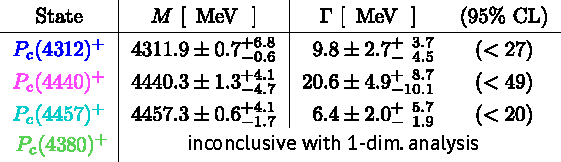
\includegraphics[width=\textwidth]{figs/PcNew/Table_1_ed.pdf}
        \end{exampleblock}
    \end{column}
    \begin{column}{0.49\textwidth}
        \vspace{-10mm}
        \begin{overlayarea}{\textwidth}{\textheight}
            \only<1>{\begin{overpic}[width=\textwidth]{figs/PcNew/mjpsip2x3.pdf}
                \put (12,35) {\tiny\color{blue}$7.6\sigma$}
                \put (30,55) {\parbox{0.2\textwidth}{
                    \tiny\centering\color{red} $5.4\sigma$\\($1$\,vs\,$2$)}}
            \end{overpic}}
            \only<2>{\vspace{7mm}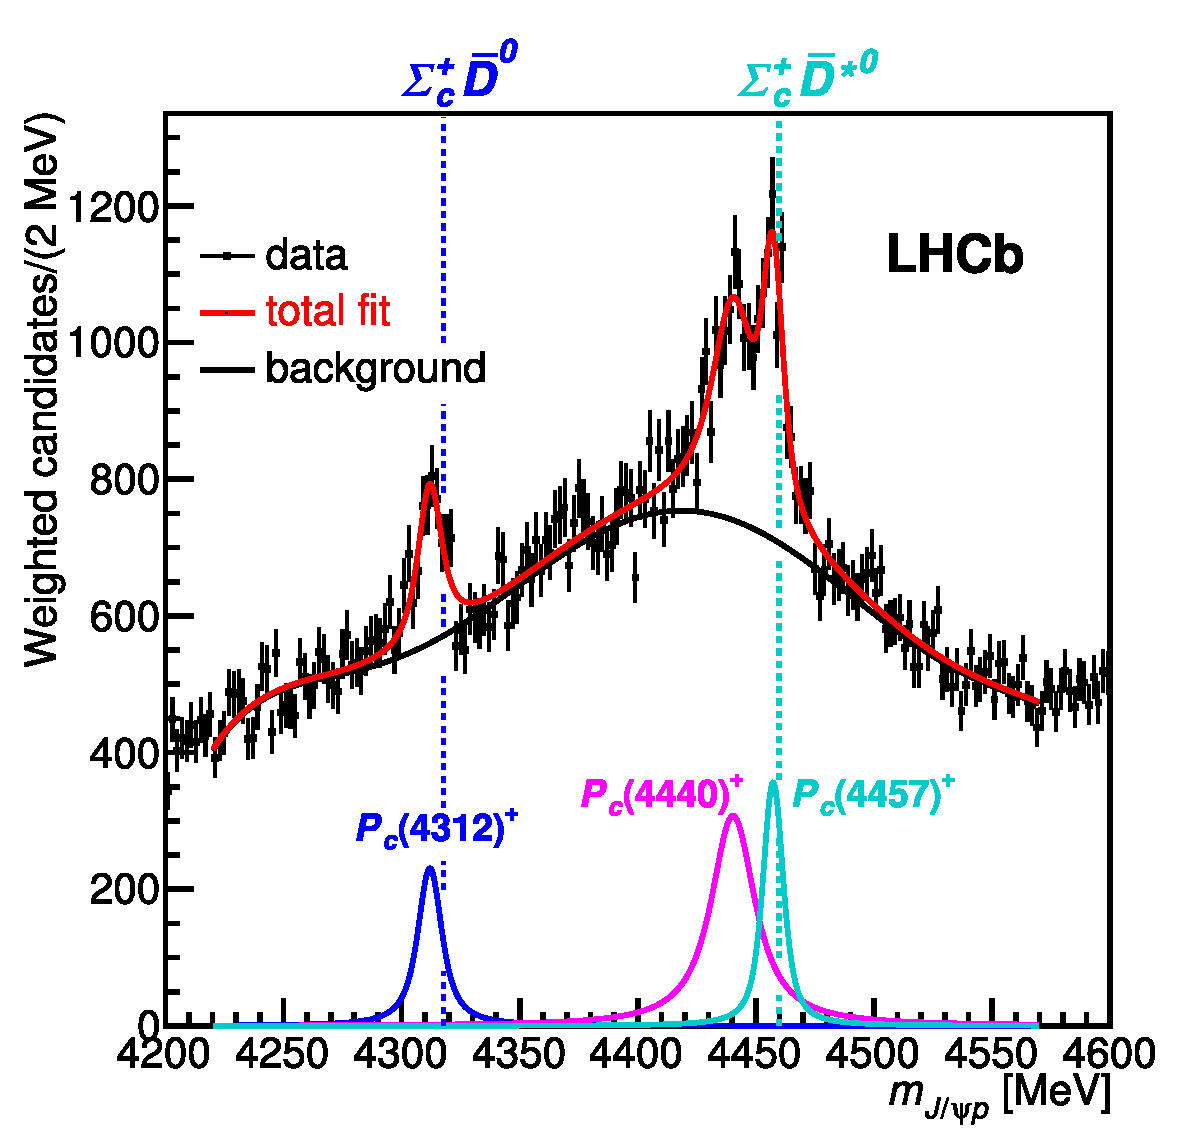
\includegraphics[width=\textwidth]{figs/PcNew/pentaquarks_nominal_fit_and_thresholds.pdf}}
            % \only<3>{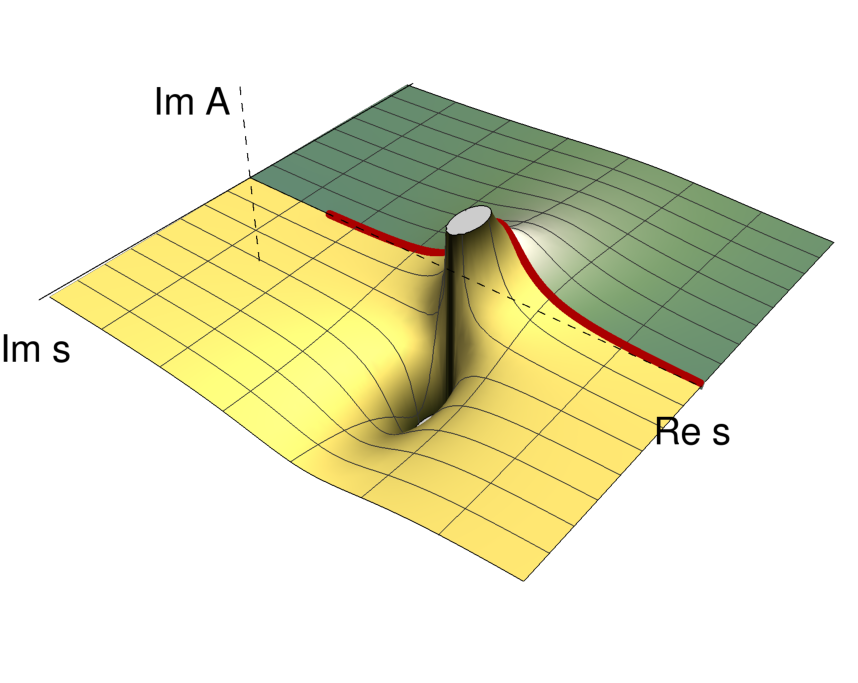
\includegraphics[width=\textwidth]{figs/sheet_2.pdf}}
        \end{overlayarea}
        % {\raisebox{-0.5\height}{
        % \begin{overpic}
        % \end{overpic}}}
        % {\vspace{5mm}\raisebox{-0.5\height}{
        % }}
    \end{column}
\end{columns}
\end{frame}

\begin{frame}{Two main interpretations of $P_c$ states}%\hfill\paper{arXiv:1904.03947}}
    \begin{columns}
        \begin{column}{0.48\textwidth}
            \begin{overpic}[width=0.9\textwidth]{figs/Pc_tigthly-bound.png}
                \put(5,2) {\color{white} tightly-bound pentaquark}
                \put(41,52) {\tiny courtesy of D.~Dominguez, CERN}
            \end{overpic}
        \end{column}
        \begin{column}{0.48\textwidth}
            \begin{overpic}[width=0.9\textwidth]{figs/Pc_molecule.png}
                \put(5,2)   {\color{white}hadronic molecule}
                \put(5,45)  {\color{white}$D^{(*)0}$}
                \put(73,3)  {\color{white}$\Sigma^{(*)+}_c$}
                \put(30,25) {\color{white}$\xLeftrightarrow[\rho,\sigma,\dots]{}$}
                %
                % \put(,25) {\color{white}$u$}
                % \put(30,25) {\color{white}$u$}
                % \put(30,25) {\color{white}$u$}
            \end{overpic}
        \end{column}
    \end{columns}
\begin{columns}
    \begin{column}{0.48\textwidth}
        \centering
        \begin{itemize}
            \item The state should have high probably to disintegrate to $J/\psi(c\bar{c})\,\, p(uud)$
            \item Diquark picture with a potential barrier \paper{Maiani et al., PLB778, 247 (2018)}
            \item Does not relate appearance to the thresholds
        \end{itemize}
        \paper{see Ref. in arXiv:1904.03947}
    \end{column}
    \begin{column}{0.48\textwidth}
        \centering
        \begin{itemize}
            \item Masses are near threshold of $\overline{D}^{0(*)} \Sigma_c^+$,
            \item Natural mechanism to separate charm quarks,
            \item Suggest importance of $\rho/\sigma$ exchanges.
        \end{itemize}
        \paper{W. L. Wang et al., Phys. Rev. C84 (2011) 015203}\\
        \paper{Z.-C. Yang et al.,  Chin. Phys. C36 (2012) 6}\\
        \paper{J.-J. Wu et al., Phys. Rev. C85 (2012) 044002}
    \end{column}
\end{columns}
\end{frame}

\begin{frame}{Pattern of states in the Heavy-Quark limit\hfill\paper{arXiv:1904.03947}}{States counting}
    \begin{columns}
        \begin{column}{0.5\textwidth}
            % \begin{center}
            %     \begin{overpic}[height=0.2\textheight]{figs/Pc_molecule.png}
            %         \put(5,2)   {\color{white}\tiny hadronic molecule}
            %         \put(5,45)  {\color{white}\small $D^{(*)0}$}
            %         \put(73,3) {\color{white}\small $\Sigma^{(*)+}_c$}
            %         \put(30,25) {\color{white}\tiny $\xLeftrightarrow[\rho,\sigma,\dots]{}$}
            %     \end{overpic}
                % \only<1>{\begin{overpic}[height=0.2\textheight]{figs/Pc_tigthly-bound.png}
                %     \put(5,2) {\color{white}\tiny tightly-bound pentaquark}
                %     \put(41,52) {\scalebox{0.3}{courtesy of D.~Dominguez, CERN}}
                % \end{overpic}}\pause
            % \end{center}\vspace{-4mm}
            \begin{block}{Heavy Quark Spin Symmetry}
                \begin{columns}
                    \begin{column}{0.3\textwidth}
                        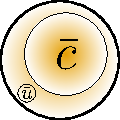
\includegraphics[width=\textwidth]{inline-figs/Meson_HQSS.pdf}
                    \end{column}
                    \begin{column}{0.7\textwidth}
                        Main interaction of $\overline{Q}q$ is strong
                        \begin{itemize}
                            \item Not sensitive to fravor
                            \item Spin-spin interaction is suppressed
                        \end{itemize}
                    \end{column}
                \end{columns}
            \end{block}
            \begin{exampleblock}{Pattern of $\Sigma_c \overline{D}$ molecules}
                % \vspace{-4mm}
            %     \begin{itemize}
            %         \item Number of states (HQSS):
            % \end{itemize}
            \vspace{-3mm}
            {\scriptsize
            \begin{align*}
                &\Sigma_c^+ \overline{D}^{0}     & 1/2^+ \otimes 0^- \xrightarrow[]{S-\text{wave}}&&& J^P:\,\color{blue}1/2^-\\
                &\Sigma_c^+ \overline{D}^{*0}    & {1}/{2}^+ \otimes 1^- \xrightarrow[]{S-\text{wave}}&&& J^P:\,{\color{purple}{1}/{2}^-}\oplus{\color{cyan}{3}/{2}^-}\\
                &\Sigma_c^{*+} \overline{D}^{*0} & {3}/{2}^+ \otimes 1^- \xrightarrow[]{S-\text{wave}}&&& J^P:\,{1}/{2}^-\oplus{3}/{2}^-\oplus{5}/{2}^-
            \end{align*}}
            \vspace{-7mm}\\
            \scriptsize
            Many theoretical predictions of $\Sigma_c\,D$ binding
            published before 2015 (see backup).
            % Relation between binding energy based on HQSS \paper{1903.11560},
            % Support from HQSS, \paper{HQSS}.\\
            % Run-III $\Rightarrow \times 3$ in statistics.
            \end{exampleblock}
            % \begin{block}{Other models}
            %     \begin{itemize}
            %         \item Tightly-bound pentaquarks
            %         \item Rescattering effects
            %     \end{itemize}
            % \end{block}
        \end{column}
        \begin{column}{0.5\textwidth}
            \centering
            \alt<2>{
            \begin{overpic}[width=0.9\textwidth]{figs/PcNew/pentaquarks_nominal_fit_and_thresholds_ed.pdf}
                \put(74,45) {\color{green!70!black} \circle{15}}
                \put(78,50) {\parbox{0.25\textwidth}{\centering\scriptsize Look forward for Run-III}}
                \put(80,80) {\parbox{0.25\textwidth}{\tiny [Ming-Zhu Liu et al., arXiv:1903.11560]}}
            \end{overpic}
            }{
            \begin{overpic}[width=0.9\textwidth]{figs/PcNew/pentaquarks_nominal_fit_and_thresholds.pdf}
            \end{overpic}
            }
            \begin{itemize}
                \item Important check is $J^{P}$ of states!
            \end{itemize}
        \end{column}
    \end{columns}
\end{frame}
%
% \begin{frame}[noframenumbering]{$P_c$ interpretations}
%     % \scalebox{0.8}{\parbox{\textwidth}{
%     \begin{itemize}
%         \item $\Sigma_c D$ binding (published before 2015)
%         % \begin{itemize}
%             % \item W. L. Wang et al., Phys. Rev. C84 (2011) 015203
%             % \item Z.-C. Yang et al.,  Chin. Phys. C36 (2012) 6
%             % \item J.-J. Wu et al., Phys. Rev. C85 (2012) 044002,
%         % \end{itemize}
%         \item Dynamically generated (see references in arXiv:1904.03947)
%         % \begin{itemize}
%         %     \item J.-J. Wu et al., Phys. Rev. Lett. 105 (2010) 232001
%         % \end{itemize}
%         \item Heavy-quark-spin-symmetry (HQSS) consequences
%         \begin{itemize}
%             \item Ming-Zhu Liu et al., arXiv:1903.11560
%             \item C.W. Xiao et al., arXiv:1904.01296
%         \end{itemize}
%         \item $P_c(4312)$ pole position and molecular binding,\\C.~Fernandez, A.~Pilloni, MM (JPAC Collaboration), arXiv:1904.10021.
%         \item Tightly-bound pentaquark models (see references in arXiv:1904.03947)
%     \end{itemize}
% \end{frame}

\section{Amplitude analysis}

\begin{frame}{Basics of amplitude analysis\hfill\paper{see great books by Gribov, Collins, Martin-Spearman}}{aka $S$-matrix theory}
    \begin{columns}
        \begin{column}{0.48\textwidth}
            \centering
            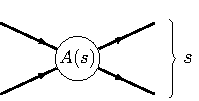
\includegraphics[width=0.6\textwidth]{inline-figs/scattering.pdf}
            \begin{exampleblock}{Scattering PW-amplitude}
                $A(s)$ is a transition amplitude
                \begin{itemize}
                    \item Complex analytic function,
                    \item Can be analytically continued to the complex energy plane,\\
                    i.e. $A(\mathrm{Re}\,s + i\,\mathrm{Im}\,s)$
                    \item The observed projection, $A(\mathrm{Re}\,s + i0)$
                \end{itemize}
            \end{exampleblock}
        \end{column}
        \begin{column}{0.5\textwidth}
            \vspace{-5mm}
            \begin{overlayarea}{\textwidth}{0.55\textheight}
                \only<1>{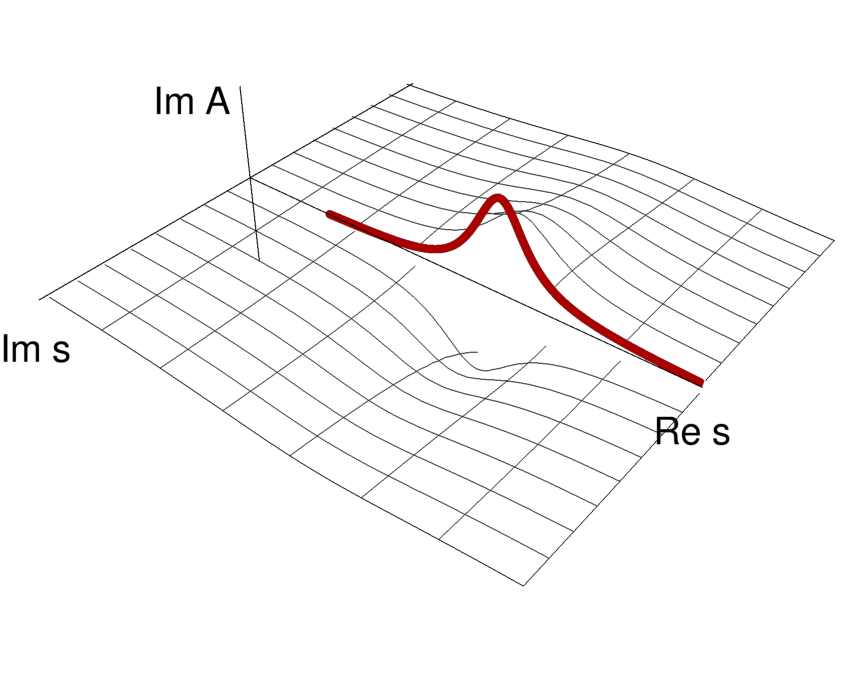
\includegraphics[width=\textwidth]{figs/sheet_0.pdf}}
                \only<2>{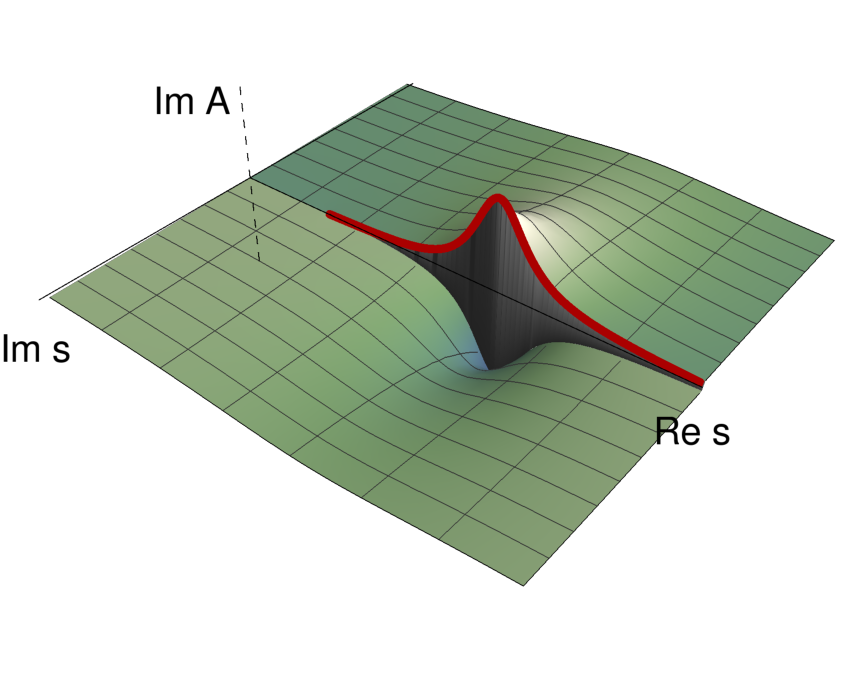
\includegraphics[width=\textwidth]{figs/sheet_1.pdf}}
                \only<3>{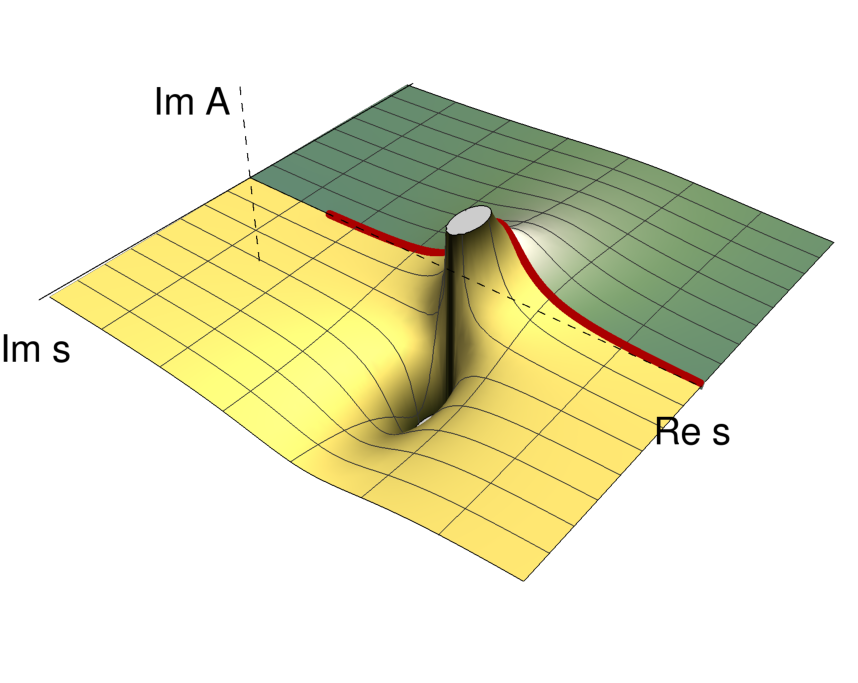
\includegraphics[width=\textwidth]{figs/sheet_2.pdf}}
                \only<4>{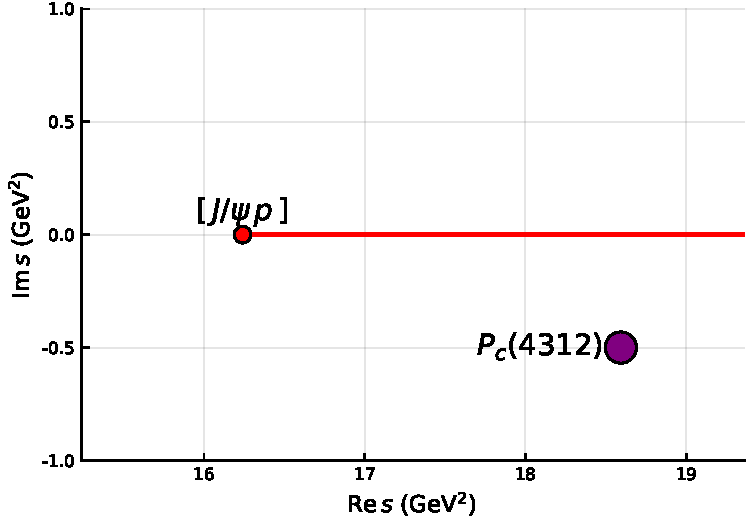
\includegraphics[width=\textwidth]{figs/Jpsi_pole.pdf}}
            \end{overlayarea}
            \begin{itemize}
                \item All structures in the energy spectum have origin in the complex plane
                \item Hadronic resonances - complex \textbf{poles}!
                \item Production thresholds - branching points.
            \end{itemize}
        \end{column}
    \end{columns}
\end{frame}

\begin{frame}{Range of interaction and different manifistation}{Model statements}
\begin{columns}
    \begin{column}{0.49\textwidth}
        \textbf{Compact state is the resonance in the $J/\psi p$ system}
        \begin{itemize}
            \item Generated by the short-range QCD forces
            \item Potential involves contact interaction
        \end{itemize}
        \centering
        \begin{overpic}[width=0.8\textwidth]{inline-figs/scattering_contact.pdf}
            \put(30,-10) {$\Rightarrow$\,\,\raisebox{-0.5\height}{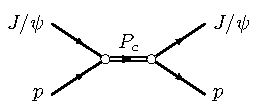
\includegraphics[width=0.5\textwidth]{inline-figs/scattering_shortrange.pdf}}}
        \end{overpic}
    \end{column}
    \begin{column}{0.49\textwidth}
        \textbf{Molecule is a bound state in the $\overline{D}^0 \Sigma_c^+$}
        \begin{itemize}
            \item Generated by the long-range forces
            \item Potential is given by exchange processes
            \item Small coupling to $J/\psi p$ to the inelastic channel.
        \end{itemize}
        \centering
        \begin{overpic}[width=0.8\textwidth]{inline-figs/scattering_exchange.pdf}
            % \put(30,-10) {$\Rightarrow$\,\,Hadronic molecule}
        \end{overpic}
    \end{column}
\end{columns}
\vspace{8mm}
\begin{exampleblock}{}
    The hypothesis are difficult to separate on the model-independent way
\end{exampleblock}
\end{frame}

\begin{frame}{Classical bound-state (molecular) picture}{Complex energy plane}
    Structures of the complex scattering amplitude correspond to physical
    \begin{center}
        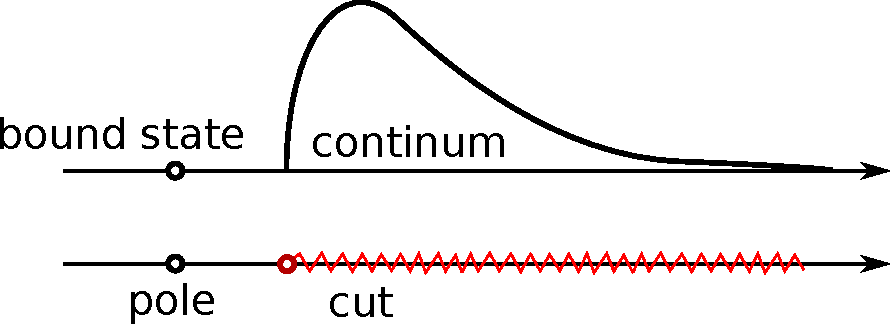
\includegraphics[width=0.6\textwidth]{figs/PcJPAC/pole_cut.pdf}
    \end{center}
    \begin{itemize}
        \item bound state - pole of the complex scattering amplitude
        \item continuum - free particles above elastic threshold (branching of the complex plane)
    \end{itemize}
\end{frame}

\begin{frame}{Strength of interaction}{Molecular bound-state vs virtual state}
    \begin{center}
        \begin{overpic}[width=0.6\textwidth]{figs/PcJPAC/pole_cut_move.pdf}
            \put(60,30) {e.g. in neutron-proton scatt. -- \textbf{deutron}}
            \put(60,0)  {e.g. in neutron-neutron scatt.}
        \end{overpic}
    \end{center}
    \begin{itemize}
        \item as weaker the binding as closer the pole to the threshold
        \item at some point moves to the unphysical sheet and leaves to $-\infty$.
    \end{itemize}
\end{frame}

\begin{frame}{Influence of the inelastic channels}{Width of the molecular state}
    \begin{center}
        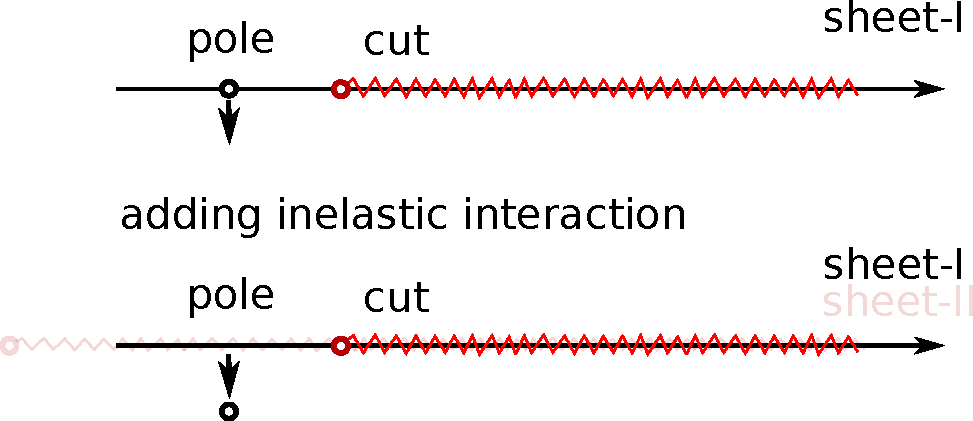
\includegraphics[width=0.7\textwidth]{figs/PcJPAC/pole_cut_inelastic.pdf}
    \end{center}
    \begin{itemize}
        \item probability to move to continuum of other channels led to shift of the pole
        \item lower threshold introduces the branching point and cut\\
        $\Rightarrow$ the pole is still on the physical sheet, causality is not violated.
    \end{itemize}
\end{frame}

\begin{frame}{Lineshape of the spectrum in the scattering length approximation}
\begin{center}
    \Huge Example demo\\[1cm]
    \raisebox{-0.5\height}{
\includegraphics[width=0.3\textwidth]{figs/julia-logo-300.png}}\qquad
    \raisebox{-0.5\height}{
\includegraphics[width=0.25\textwidth]{figs/atom_ed.png}}
\end{center}
\end{frame}

\begin{frame}{$P_c(4312)$ in molecular picture\hfill\paper{C.~Fernandez, A.~Pilloni, MM (JPAC) arXiv:1904.10021}}{Fit to the LHCb data}
\begin{columns}
    \begin{column}{0.47\textwidth}
        \begin{center}
            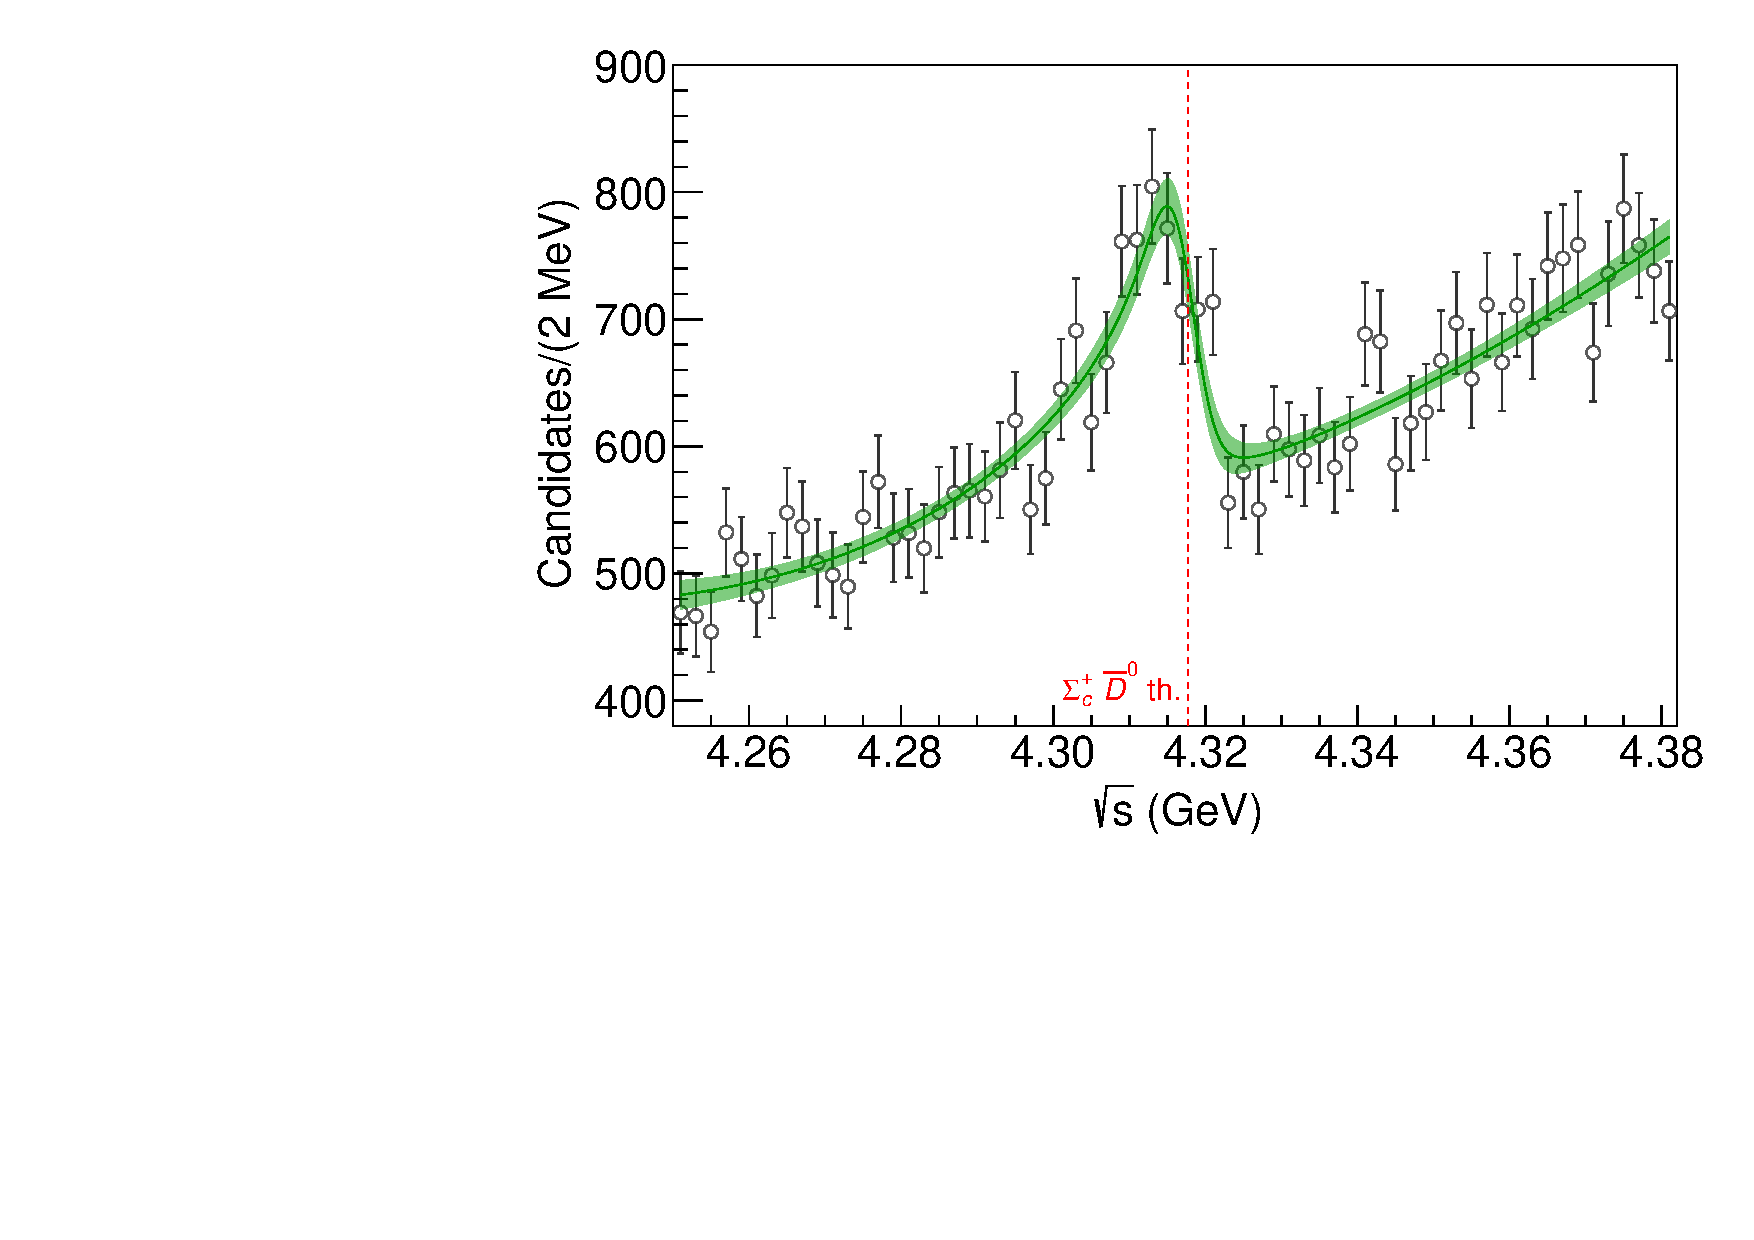
\includegraphics[width=\textwidth]{figs/PcJPAC/plot_nc.pdf}
        \end{center}
        Fit parameters:
        \begin{itemize}
            \item $m_{11}$, $m_{22}$, $m_{12}=m_{21}$,
            \item $p_0$, $p_1$, $b_0$, and $b_1$.
        \end{itemize}
    \end{column}
    \begin{column}{0.47\textwidth}
        \begin{block}{Scattering-length approximation}
            \begin{align*}
                T^{-1}_{ij} &= m_{ij} - i k_i \delta_{ij},\\
                k_i &= \sqrt{s-s_i}
            \end{align*}
            Two channels: $\Sigma_c^+ \bar{D}^0$ and $J/\psi p$.
        \end{block}
        \begin{exampleblock}{Intensity}
            \vspace{-3mm}
            $$
            I(s) = \rho(s)(|T_{11}(s) \,p(s)|^2 + b(s)),
            $$
            \vspace{-5mm}
            \begin{itemize}
                \item $p(s)$ and $b(s)$ are the first order polynomials.
                \item $\rho(s)$ is a phase-space factor.
            \end{itemize}
        \end{exampleblock}
    \end{column}
\end{columns}
\end{frame}

\begin{frame}{Pole position of the $P_c(4312)$ state\hfill\paper{arXiv:1904.10021}}
\begin{columns}
    \begin{column}{0.67\textwidth}
        \begin{overpic}[width=\textwidth]{figs/PcJPAC/general_nc_ed.pdf}
            \put(40,50) {\color{green!60!black}$\text{Im}(\gamma) = m_{12}\to 0$}
        \end{overpic}
    \end{column}
    \begin{column}{0.3\textwidth}
        \begin{itemize}
            \item Large uncertainties to the pole position due to statistical uncertainties
            \item Obtained parameters suggest $P_c(4312)$ to be a \textbf{virtual state}
            \item When coupling $m_{12}$ is turned off, the pole ends up on the unphysical sheet
        \end{itemize}
        % \includegraphics[width=0.5\textwidth]{figs/PcJPAC/general_nc_ed.pdf}
    \end{column}
\end{columns}
\end{frame}

\begin{frame}[plain]{}{}
\begin{columns}
    \begin{column}{0.6\textwidth}
        {\Large \color{cola}
         Hadrons are confined colors of QCD!}
        % \vspace
        \begin{exampleblock}{Hadron spectroscopy}
            \begin{itemize}
                \item is an active field with ground-breaking discoveries,
                \item with many players and approaches:
                \begin{itemize}
                    \item Experiments (LHCb, Belle, BESIII, COMPASS, GlueX, $\dots$)
                    \item Lattice QCD (HadSpec, BMW, $\dots$)
                    \item Phenomenological potential models
                    \item Amplitude Analysis
                \end{itemize}
            \end{itemize}
        \end{exampleblock}
        % \vspace{1cm}
        \begin{block}{Pentaquarks are new formations of the matter}
            \begin{itemize}
                \item The existence is confirmed \quad {\small(c) LHCb}.
                \item A pattern of the new spectroscopy sector is emerging
            \end{itemize}
        \end{block}
    \end{column}
    \begin{column}{0.38\textwidth}
        \includegraphics[width=\textwidth]{figs/buckets.jpg}
    \end{column}
\end{columns}
\end{frame}

{\usebackgroundtemplate{\includegraphics[width=\paperwidth]{figs/paint-strokes_smaller.jpg}}
\begin{frame}[plain,noframenumbering]{}{}
    \begin{center}
        \transparent{0.7}
        \colorbox{white}{
        \transparent{1}
        \parbox{0.8\textwidth}{
        \centering
        \Huge Thank you for the attention
        }}
    \end{center}
\end{frame}
}

\begin{frame}[plain,noframenumbering]{}{}%{Pentaquarks and Tetraquarks}
    \centering
    \begin{overpic}[width=0.95\textwidth]{figs/SPONGE-BOB-AND-PATRICK-STAR-RUNNING-poster.jpg}
        \put (5,2) {\Large Follow the \textbf{Pentaquark} and \textbf{Tetraquark} investigation!}
    \end{overpic}
\end{frame}

%%%%%%%%%%%%%%%%%%%%%%%%%%%%%%%%%%%%%%%%%%%%%%%%%%%%%%%%%%%%%%%%%%%%%%%%%%%%%%%
%%%%%%%%%%%%%%%%%%%%%%%%%%%%%%%%%%%%%%%%%%%%%%%%%%%%%%%%%%%%%%%%%%%%%%%%%%%%%%%
%%%%%%%%%%%%%%%%%%%%%%%%%%%%%%%%%%%%%%%%%%%%%%%%%%%%%%%%%%%%%%%%%%%%%%%%%%%%%%%
%%%%%%%%%%%%%%%%%%%%%%%%%%%%%%%%%%%%%%%%%%%%%%%%%%%%%%%%%%%%%%%%%%%%%%%%%%%%%%%

\begin{frame}[noframenumbering]{Rescattering interpretation}%{Triangle singularity {\scriptsize [see Appendix of arXiv:1904.03947]}}
\begin{columns}
    \begin{column}{0.58\textwidth}
        \vspace{-1mm}
        \begin{center}
            \includegraphics[width=0.5\textwidth]{figs/PcNew/triangle.png}
        \end{center}
        \vspace{-2mm}
        \begin{itemize}
            \item There are many thresholds around $P_c$ peaks
            \begin{itemize}
                \item $\Lambda_c \bar{D}^0$, $\Sigma_c \bar{D}^0$, $\chi_c\,N^*$ with different exchanges\\
                as suggested in \paper{Guo et al.(PRD92 (2015) 071502), U.-G. Meißner et al. (PLB751 (2015) 59), X.-H. Liu et al. (PLB757 (2016) 231), MM (arXiv:1507.06552)}
            \end{itemize}
            \item An appropriate Triangle Singularity can be found for all peaks
            \item BUT, as soon as \textbf{width} of exchange particle is taken into account
        \end{itemize}
        % \vspace{8mm}
        $\Rightarrow$ no acceptable description in rescattering picture have been found
    \end{column}
    \begin{column}{0.4\textwidth}
        \vspace{-1cm}
        \begin{overpic}[width=\textwidth]{figs/PcNew/triangleFits.pdf}
        \end{overpic}
    \end{column}
\end{columns}
\end{frame}

\begin{frame}[noframenumbering]{Scattering amplitude}{(see e.g. Landau and Lifshitz, Vol.III, (132.9))}
$D\overline{D}^* \to D\overline{D}^*$ scattering. $T(s)$ is $S$-wave scattering amplitude
\begin{equation*}
    T(s)
    = \overbrace{-\alpha}^{\text{scattering length}}
    = \underbrace{\frac{1}{-\gamma}}_{\gamma \text{ is the inverse scattering length}}
\end{equation*}
Energy dependence in vicinity of threshold, $m_\text{th} = m_D+m_{D^*}$:
\begin{equation*}
    T(s) = \underbrace{\frac{1}{-\gamma-i k}}_{\text{momentum}~k = \frac{1}{2}\sqrt{s-s_\text{th}}} \approx
    % \underbrace{
        \frac{1}{-\gamma-i\sqrt{2\mu\,(\sqrt{s}-m_\text{th})}}
    \xrightarrow[\text{rotate cut}]{-i\sqrt{x} =+\sqrt{-x}}
    % }_{\text{rotate cut }-i\sqrt{x} =+\sqrt{-x}}
    \underbrace{
        \frac{1}{-\gamma+\sqrt{-2\mu E}}
        }_{\tiny[\text{used in PRD76 044028}]}
\end{equation*}
\begin{itemize}
    \item $\mu$ is a reduced mass, $1\mu  = 1/m_D + 1/m_{D^*}$,\\
    \item $E = \sqrt{s}-m_\text{th}$ is a distance from threshold
\end{itemize}
\end{frame}


\begin{frame}[noframenumbering]{Case B: effective-range model}%{}
\begin{columns}
    \begin{column}{0.4\textwidth}
        \begin{center}
            \includegraphics[width=0.9\textwidth]{figs/PcJPAC/plot_yc.pdf}\\
            \includegraphics[width=0.9\textwidth]{figs/PcJPAC/general_yc.pdf}
        \end{center}
    \end{column}
    \begin{column}{0.57\textwidth}
        \begin{block}{Effective-range approximation}
            \begin{align*}
                T^{-1}_{ij} &= m_{ij} + {\color{red} c_{ij} s} - i k_i \delta_{ij},\\
                k_i &= \sqrt{s-s_i}
            \end{align*}
            Two channels: $\Sigma_c^+ \bar{D}^0$ and $J/\psi p$.
        \end{block}
        \begin{exampleblock}{Fit parameters}
            \begin{itemize}
                \item $m_{11}$, $m_{22}$, $m_{12}=m_{21}$, $c_{11}$, $c_{22}$
                \item $p_0$, $p_1$, $b_0$, and $b_1$.
            \end{itemize}
        \end{exampleblock}
    \end{column}
\end{columns}
\end{frame}

\begin{frame}[noframenumbering]{Three channels: effective-range model}%{}
\begin{columns}
    \begin{column}{0.4\textwidth}
        \begin{center}
            \includegraphics[width=0.9\textwidth]{figs/PcJPAC/plot_3nc.pdf}\\
            \includegraphics[width=0.9\textwidth]{figs/PcJPAC/general_3nc.pdf}
        \end{center}
    \end{column}
    \begin{column}{0.57\textwidth}
        \begin{block}{Effective-range approximation}
            \begin{align*}
                T^{-1}_{ij} &= m_{ij} + - i k_i \delta_{ij},\\
                k_i &= \sqrt{s-s_i}
            \end{align*}
            Two channels: $\Sigma_c^+ \bar{D}^0$, $\Sigma_c^{++} \bar{D}^-$ and $J/\psi p$.
        \end{block}
        \begin{exampleblock}{Fit parameters}
            \begin{itemize}
                \item $m_{11}$, $m_{22}$, $m_{12}=m_{13}$, $m_{23}$, $c_{11}$, $m$ is symmetric.
                \item $p_0$, $p_1$, $b_0$, and $b_1$.
            \end{itemize}
        \end{exampleblock}
    \end{column}
\end{columns}
\end{frame}

\begin{frame}[noframenumbering]{Systematic studies}
\begin{itemize}
    \item Other data samples: cut $M_{Kp}>1.9\,$GeV, all-$Kp$.
    \item Extended model(see backup)
    \begin{itemize}
        \item case B: effective-range expansion $m_{ij} \to m_{ij}+c_{ij} s$
        \item including third channel $(\Sigma_c^{++} D^-$.
        \item tests of K-matrix parametrization and the Flatte parametrization
    \end{itemize}
\end{itemize}
\end{frame}

\end{document}
